\chapter{Methods}\label{sec:methods}
In this chapter, the methods for investigating a bridge design, verifying its structural safety and estimating its cost are introduced. In Section \ref{sec:met_ref} the Blennerhassett Island Bridge, as well as other reference bridges, are presented.
Section \ref{sec:met_str} introduces the structural model and briefly assesses its underlying assumptions. Further, an overview of the investigated load cases is given in Section \ref{sec:met_loads}. The determination of the self-equilibrium stress state is of critical importance. The designer can freely assign it to the structure, contrary to the load cases, whose effects are determined by the elastic response of the structure. Section \ref{sec:met_seq} describes different methods to obtain this state which also includes the choice of the arch shape. The limit states for the design criteria as well as the corresponding verifications are specified in Section \ref{sec:met_ver}, combining the self-equilibrium stress state with the factored load cases. Based on these verifications, the cost of an investigated design is estimated according to Section \ref{sec:met_cost}. The methods presented in this chapter are exemplified by the final design of the Blennerhassett Island Bridge based on the design drawings.

\section{Reference bridges} \label{sec:met_ref}

\newpage
\section{Structural model} \label{sec:met_str}
A defining feature of the Blennerhassett Island Bridge is the floating deck. It is supported only at the 13 floor beams and acts almost structurally independent and resembles a bridge by itself. Compared to a composite deck, it causes a certain inefficiency in material use and the additional arrangement of many bearings. On the other hand, it allows for a replacement of the deck in the future and it simplifies the investigation of the flow of forces. It carries the loads over a span of 20 meters to the adjacent floor beams. There, the forces are mainly carried by the respective hanger pair and partially by the tie girder. This feature allows for a separation of the behaviour of the remaining network arch from the deck. As it is not the objective of this Thesis to investigate and optimise the deck system it is not further considered. The structural model of the network tied-arch bridge is therefore composed of the tie, the arch and the hangers. According to Smit, the behaviour of the two planes of the arch can be considered decoupled from each other \cite{Smit}. Therefore, the behaviour of the arch is analysed in a single arch plane. In the design drawings, the structure is divided into segments for the arch and the tie. Each of these segments is verified independently in the design verifications. This segmentation, which is shown along with the bridge in Figures \ref{fig:Blennerhassett2_a} and \ref{fig:fig:Blennerhassett2_b}, is also used for the analysis in this Thesis.

\begin{figure}[H]
\centering
\begin{subfigure}{0.5\textwidth}
    \centering
    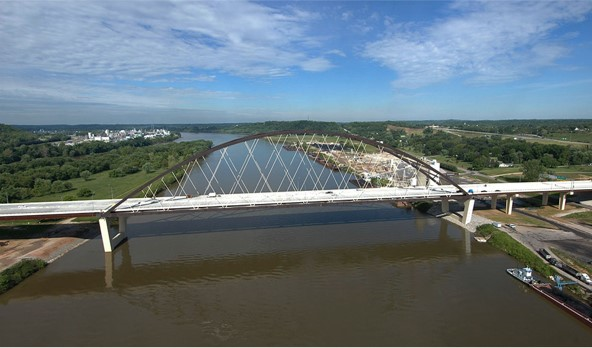
\includegraphics[width=0.9\textwidth]{overleaf/Pictures/Blennerhassett_2.jpg}
    \caption{Built structure}
    \label{fig:Blennerhassett2_a}
\end{subfigure}%
\begin{subfigure}{.5\textwidth}
    \centering
    \vspace*{0.67cm}
    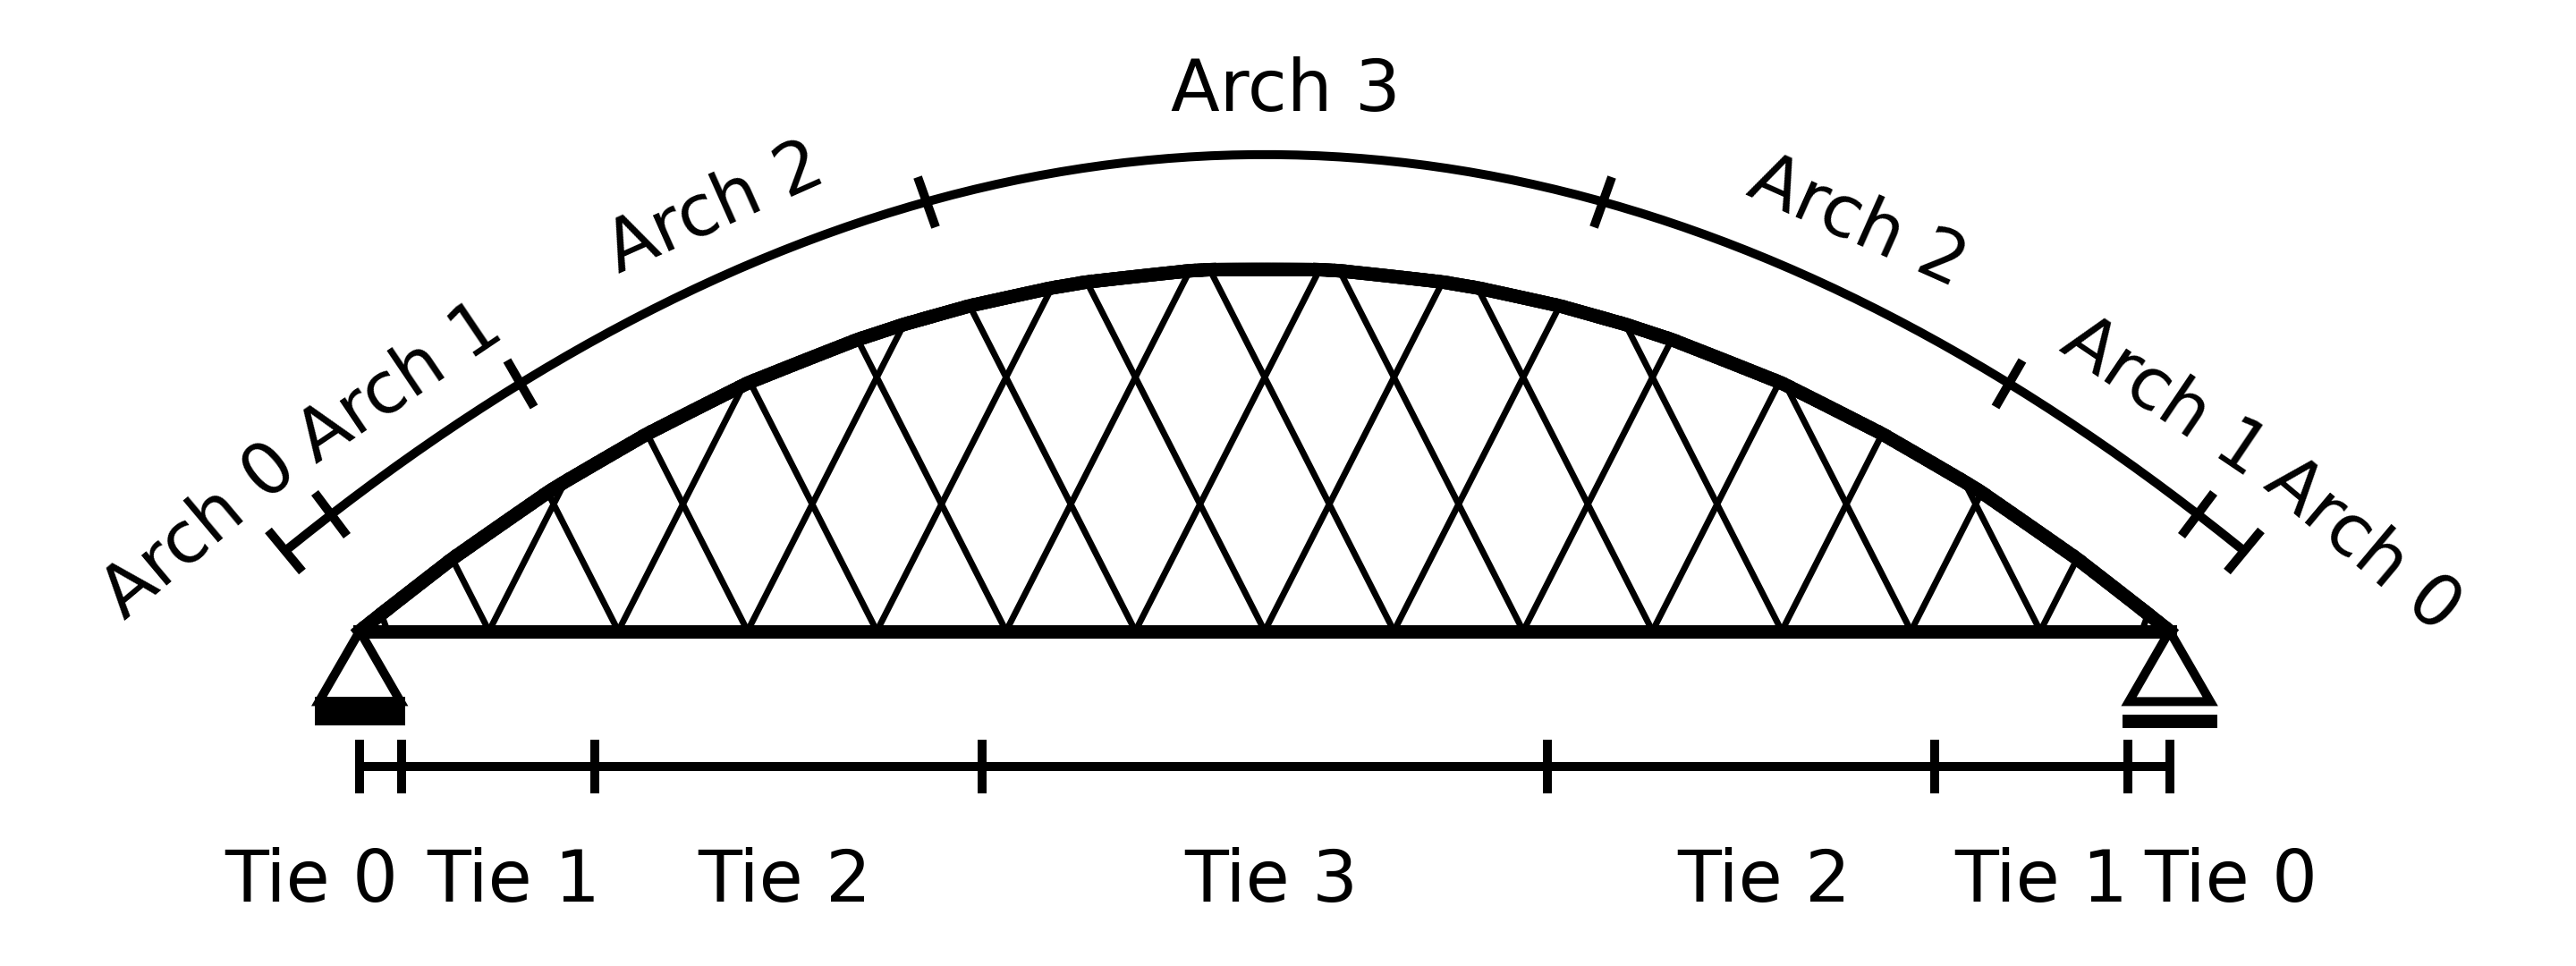
\includegraphics[width=0.9\textwidth]{illustrations/figures/segments.png}
    \vspace*{0.67cm}
    \caption{Structural model and segments}
    \label{fig:fig:Blennerhassett2_b}
\end{subfigure}
\caption{Blennerhassett Island Bridge}
\label{fig:Blennerhassett2}
\end{figure}

Both the arch and the tie girder feature are a box cross-section with a width of \SI{1.2}{m}. The one of the arch is \SI{1.7}{m} high and offers similar bending resistances around both axes. Additionally, it is reinforced by a web stiffener to prevent local buckling. The cross-section of the tie girder is \SI{2.2}{m} high and offers more resistance for longitudinal than transverse bending moments. Both the arch rib and the tie girder feature a stronger cross-section in the knuckle region, where the highest internal force effects are expected. The segments Arch 0 and Tie 0 form the knuckle and are assigned the strongest cross-sections, with resistances about 50\% higher than in the field. They are not subject to the optimisation in this Thesis as they cannot accurately be dimensioned as beam elements. Also the next segments Arch 1 and Tie 1 have a slightly enhanced cross-section with thicker plates. The remaining segments in the field feature identical cross-sections for the tie girder and the arch rib respectively. They are considered the characteristic cross-sections and are shown in Figures \ref{fig:cs_arch} and \ref{fig:cs_tie}. All cables have identical cross-sections with 29 high-strength strands of \SI{140}{mm^2}. The respective lengths range from \SI{11}{m} to \SI{59}{m}. The corresponding cross-section including its tube is shown in Figure \ref{fig:cs_cable}. The most important properties are specified in Table \ref{tab:cs_properties}. More detailed specifications on the cross-sections are found in the Appendix \ref{app:cross_sections}.

\begin{figure}[H]
\centering
\begin{subfigure}{0.33\textwidth}
    \centering
    \vspace*{0.68cm}
    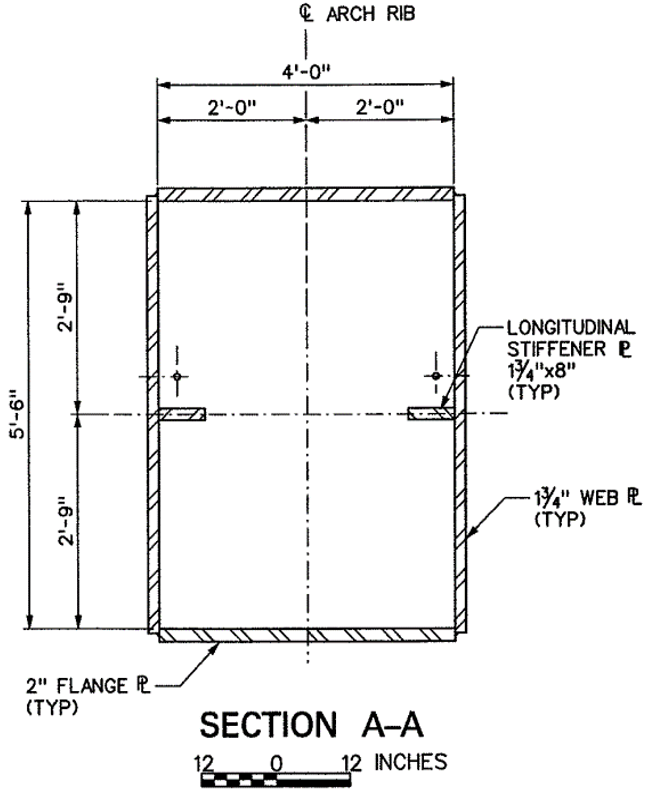
\includegraphics[width=0.8\textwidth]{overleaf/Appendix/Pictures/arch_3.PNG}
    \vspace*{0.68cm}
    \caption{Arch rib}
    \label{fig:cs_arch}
\end{subfigure}%
\begin{subfigure}{.33\textwidth}
    \centering
    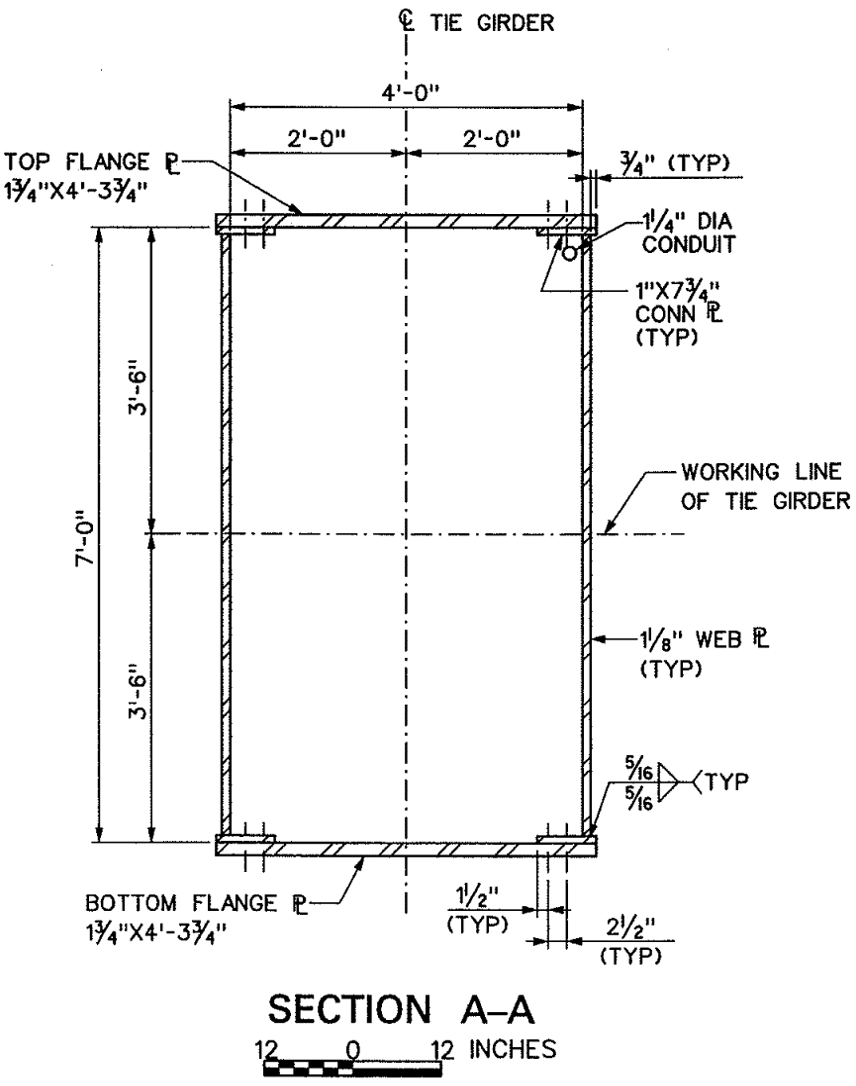
\includegraphics[width=\textwidth]{overleaf/Appendix/Pictures/tie_3.PNG}
    \caption{Tie girder}
    \label{fig:cs_tie}
\end{subfigure}%
\begin{subfigure}{.33\textwidth}
    \centering
    \vspace*{1.35cm}
    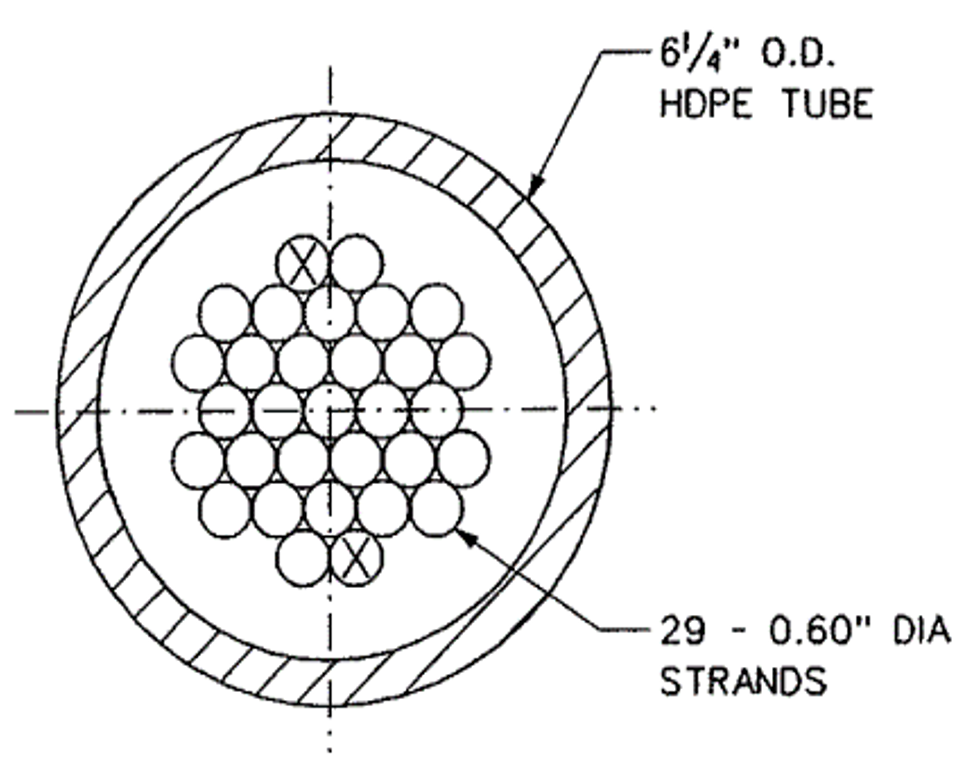
\includegraphics[width=0.9\textwidth]{overleaf/Appendix/Pictures/cable_3.PNG}
    \vspace*{1.35cm}
    \caption{Cable}
    \label{fig:cs_cable}
\end{subfigure}\caption{Cross-sections in the field}
\label{fig:cross_sections}
\end{figure}

\begin{table}[H]
    \centering
    \caption{Properties of the field cross-sections}
    \label{tab:cs_properties}
    \begin{tabular}{lccccc}
    \toprule
    Cross-section & $EA$ & $EI$ & $N_{Rd}$ & $M_{Rd,z}$ & $M_{Rd,y}$ \\
                  & [\SI{}{GN}]   & [\SI{}{GNm^2}]   & [\SI{}{MN}]  & [\SI{}{MNm}]  & [\SI{}{MNm}] \\ \midrule
    Arch 2 \& Arch 3 & 61.8 & 28.1 & 82.3 & 50.0 & 42.7 \\
    Tie 2 \& Tie 3  & 53.7 & 42.8 & 100.5 & 76.2 & 45.8 \\
    Cables        & 0.8 &  - & 6.8 & - & - \\ \bottomrule
    \end{tabular}
\end{table}

Considering their slenderness, the arch and the tie can be accurately modelled as beam elements. On the other hand, secondary effects cannot always be neglected for the hangers because of their low bending stiffness. However, a brief investigation, given in Appendix \ref{Appendix_A_Hangers}, shows that above \SI{100}{MPa} these effects are irrelevant. Therefore, the hangers are modelled as beams with rotational end releases and their self-weight is neglected. Additionally, two web plates connecting the tie girder and the arch rib in the knuckle region are arranged to obtain a more accurate representation of this detail. Each web plate has a cross section of \SI{6.3}{cm} x \SI{1.07}{m} and is arranged \SI{4.1}{m} for the idealised node at an angle of 80\degree. The web plates are illustrated in Figure \ref{fig:knuckle_region}.



\begin{figure}[H]
    \centering
    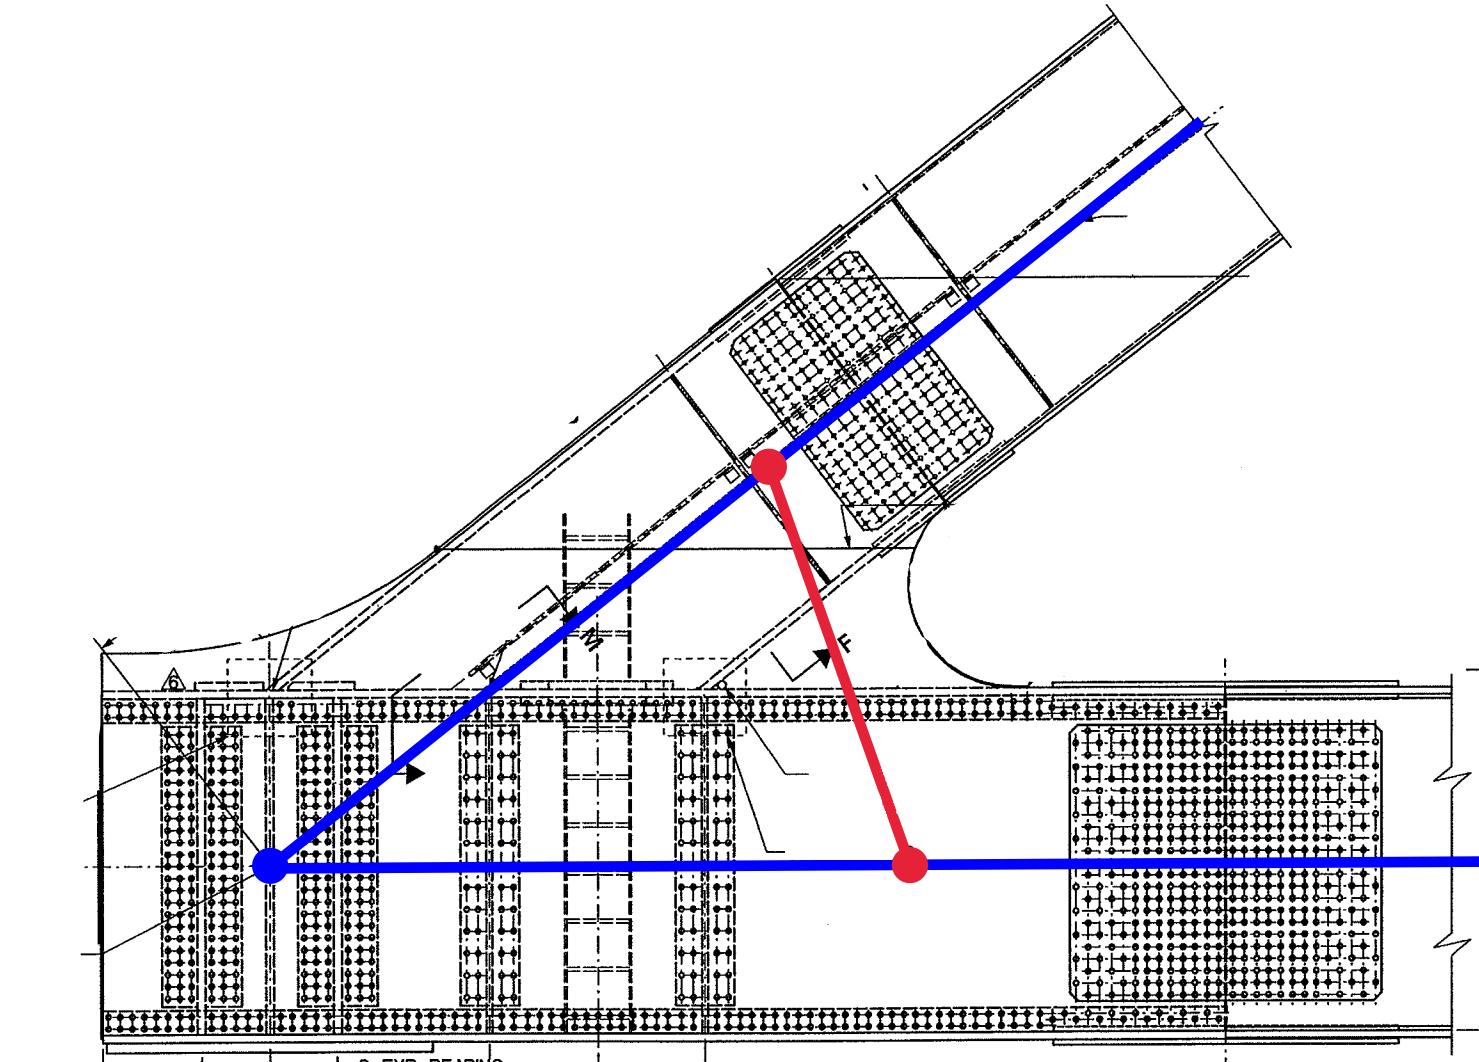
\includegraphics[width=0.5\textwidth]{overleaf/Pictures/Knuckle region.png}
    \caption{Plan and structural model of the knuckle region}
    \label{fig:knuckle_region}
\end{figure}

The structure is analysed in the framework of two-dimensional and linear elastic beam statics. Therefor, a python package written by the author in an earlier project is used. It is verified with the Sofistik model of a parallel Master Thesis in Appendix \ref{app:model_verification}. To judge the dependency of the resulting internal force effects on the described modelling, the structure is first analysed using different simplified models. In the first simplistic model, the field cross-sections are used everywhere and also no web member is considered. In a second model, the previously described web plated are introduced. Additionally, the actual cross-sections are assigned to the arch and the tie in a third model. The elastic effects under dead loads are compared in Figure \ref{fig:model_comparison}.

\begin{figure}[H]
    \centering
    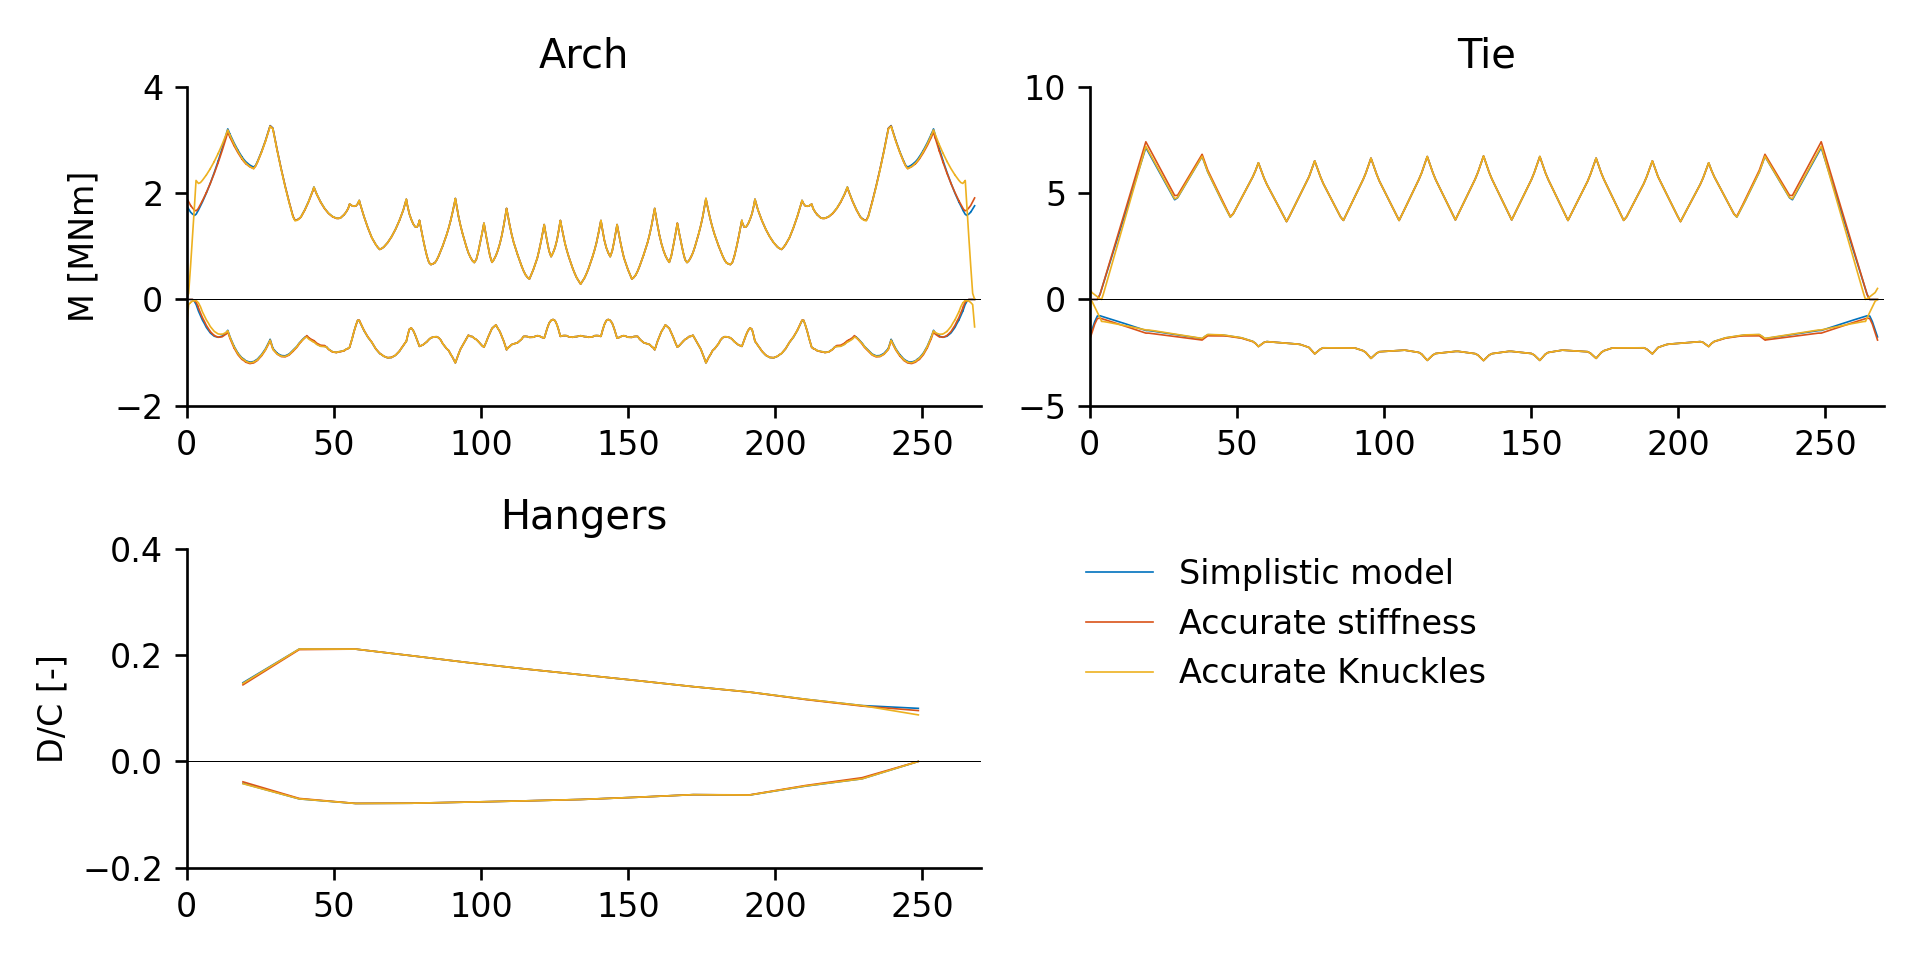
\includegraphics[width=0.9\textwidth]{calculations/model comparison/live_loading.png}
    \caption{Comparison of the elastic responses under live loading for different models}
    \label{fig:model_comparison}
\end{figure}

[Conclusion]

\newpage
\section{Load cases} \label{sec:met_loads}
The load cases relevant to this investigation are the dead loading (DL), the live loading (LL) and the wind loading (WS). The dead loading is further subdivided into the weight of the structural components and non-structural attachments (DC) and the weight of the future wearing surfaces and utilities (DW).

\subsection{Dead loading}
The dead loads for the Blennerhassett Island Bridge were derived from the estimated bridge quantities of the design drawings. The detailed derivation is given in Appendix \ref{app:weight} and the final results are presented in Table \ref{tab:dead_loads}. The weight of the arch and the tie girder are distributed as a constant load along the respective elements. A particularly detailed weight distribution by assigning more weight to the stronger cross-sections near the knuckle is disregarded for. Also the weight of the lateral arch bracing is distributed along the entire arch for simplicity. The deck weight and its non-structural components make up for the main contribution to the dead loading. The weight of the deck is applied as a concentrated force at the locations of the floor beams. The weight of the hangers and its resulting bending moment is relatively small and neglected to facilitate some of the used optimisation methods. An illustration of all dead loads applied to the structural model is shown in Figure \ref{fig:dead_loads}.

\begin{table}[H]
    \centering
    \caption{Weights of the structural and non-structural components}
    \label{tab:dead_loads}
    \begin{tabular}{lcccc}
        \toprule
        Component & Arch & Tie & Deck & Utilities \\ \midrule
        Weight & \SI{29.8}{kN/m} & \SI{26.4}{kN/m} & \SI{115.3}{kN/m} & \SI{35.1}{kN/m} \\ \bottomrule
    \end{tabular}
\end{table}

\begin{figure}[H]
    \centering
    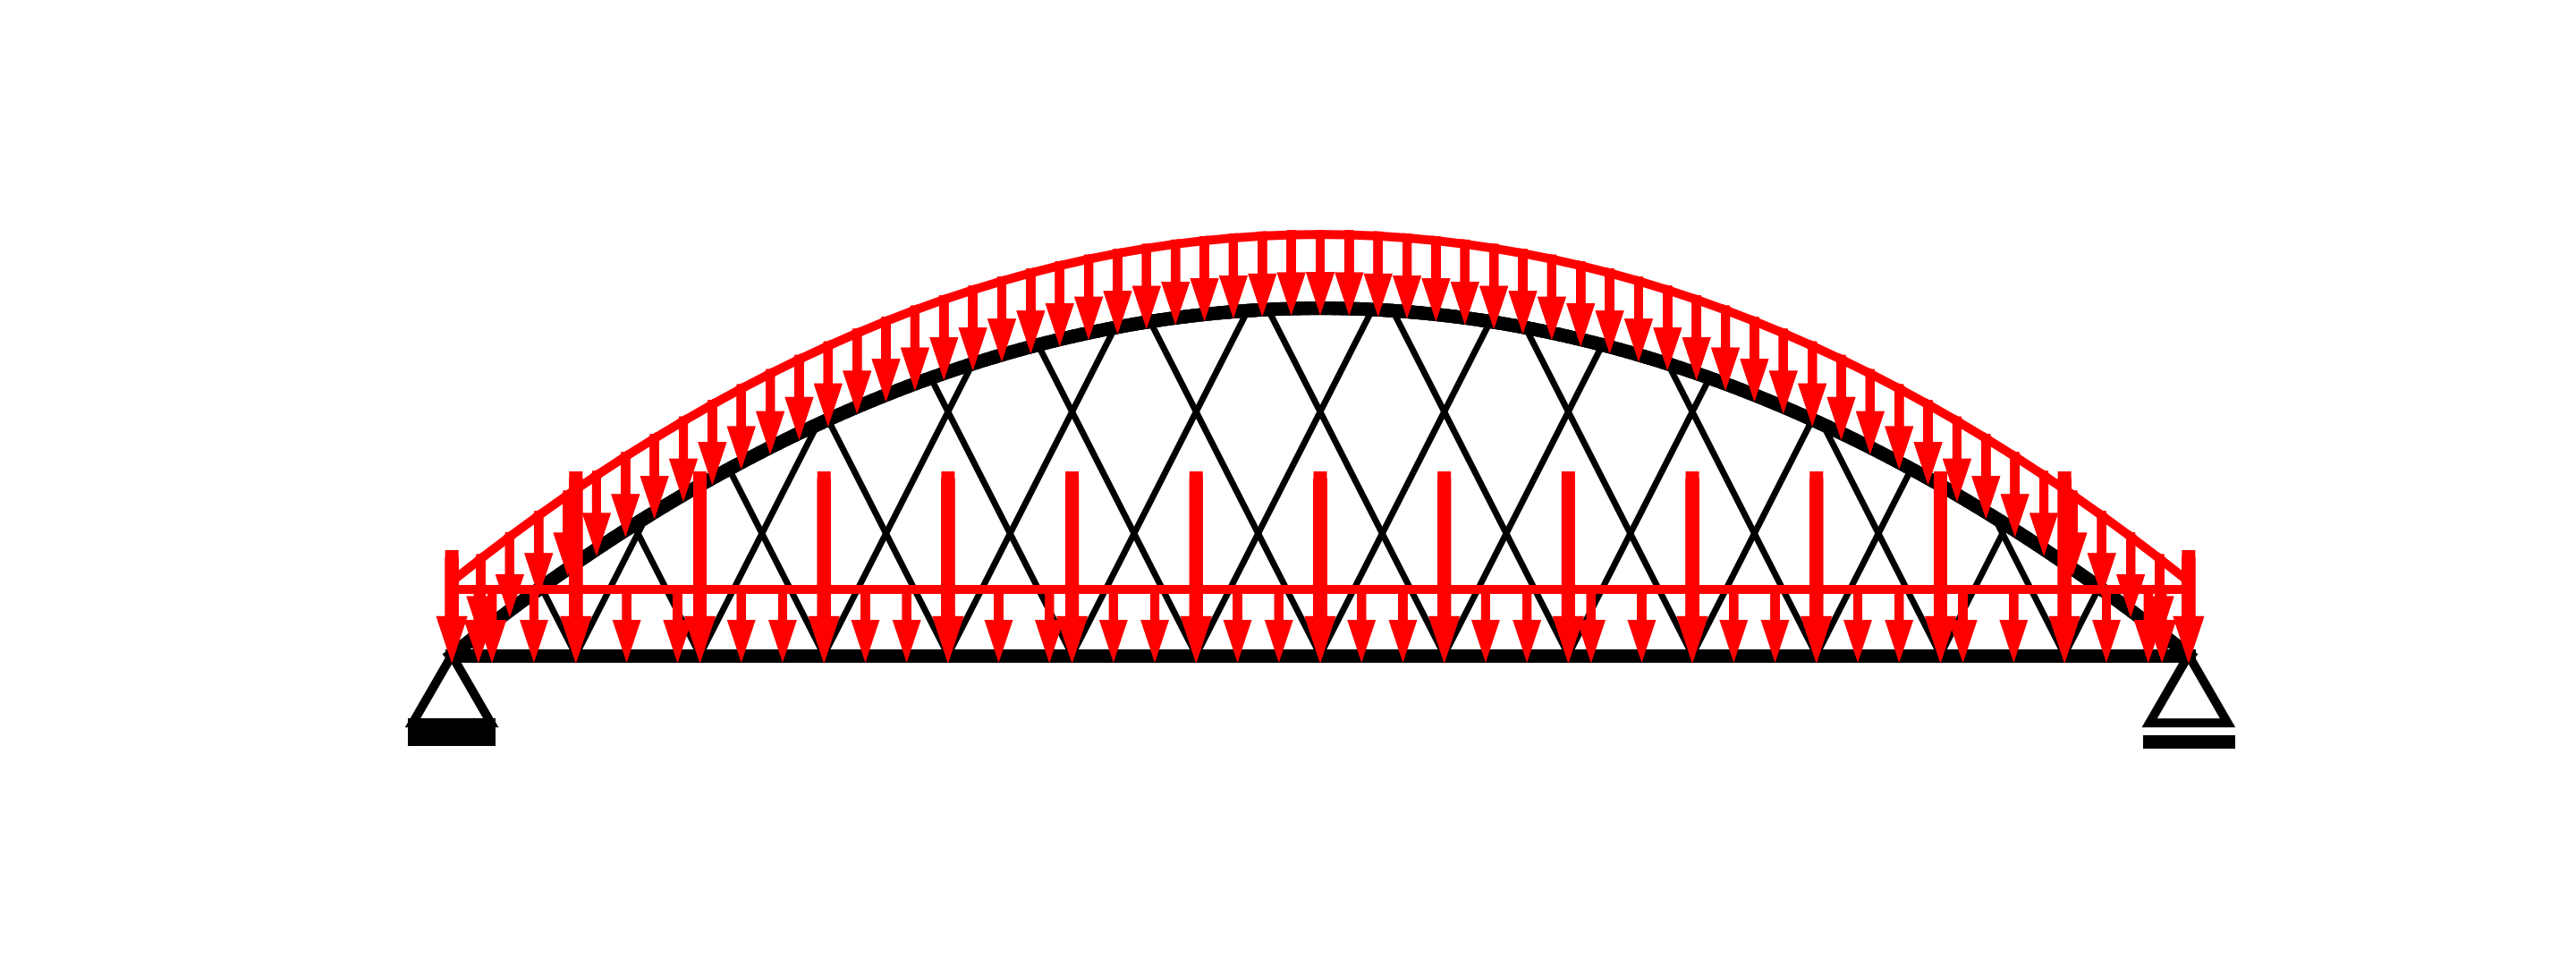
\includegraphics[trim={0 0.8cm 0 0.8cm},clip,
    width=0.8\textwidth]{illustrations/figures/permanent loads.png}
    \caption{Dead loading in the structural model}
    \label{fig:dead_loads}
\end{figure}

\subsection{Live loading} \label{sec:met_loads_live}
The load case of live loading is taken into account according to the AASHTO Bridge Design Specifications (1998) \cite{AASHTO}. It is a combination of two separate components: A lane-wise distributed load is applied along the entire or partial length of the bridge and a concentrated truck load is applied at a single longitudinal point. Both loads are factored by a multiple presence factor (MPF) depending on how many lanes are loaded. In a detailed calculation in Appendix \ref{Appendix_Liveloading}, six loaded lanes were found to cause the highest load in the considered arch plane. This conclusion also applies to the truck loads, which are also applied simultaneously on six lanes. An overview of the design loads is given in Table \ref{tab:live_load_overview}. 

\begin{table}[H]
\centering
\caption{Overview of the live loading}
\label{tab:live_load_overview}
\begin{tabular}{cccccc}
\begin{tabular}[c]{@{}c@{}}Design\\ lane load\end{tabular} & \begin{tabular}[c]{@{}c@{}}Design\\ truck weight\end{tabular} & \begin{tabular}[c]{@{}c@{}}Lane\\ multiplier\end{tabular} & \begin{tabular}[c]{@{}c@{}}Dynamic\\ multiplier\end{tabular} & \begin{tabular}[c]{@{}c@{}}Distributed\\ design load\end{tabular} & \begin{tabular}[c]{@{}c@{}}Concentrated\\ design load\end{tabular} \\ \hline
\SI{9.3}{kN/m} & \SI{325}{kN} & \SI{2.46}{} & \SI{1.33}{} & \SI{23.0}{kN/m} & \SI{1063}{kN}
\end{tabular}
\end{table}


The live loads are applied on the deck, which is not part of the structural model. Therefore, the live loads act as concentrated forces on the floor beams, where the deck is supported, as illustrated in Figures \ref{fig:Live_load_1} for the fully loaded deck. To find the worst arrangement of the live loads, the concentrated forces are applied individually. For each point of interest in the model, the partially distributed lane load and the concentrated truck force are then combined to produce maximum effects. The concentrated force is thereby only applied at one cross-girder exclusively, as shown in Figure \ref{fig:Live_load_2}. 

%It yields a range of possible effects for each point on the structural elements. The resulting ranges for the Blennerhassett Island Bridge are presented in Figure [], where the ranges of the concentrated load and the distributed loads are also shown individually. These results agree well with the effects specified on the design drawings.\bigskip

\begin{figure}[H]
\centering
\begin{subfigure}{0.5\textwidth}
    \centering
    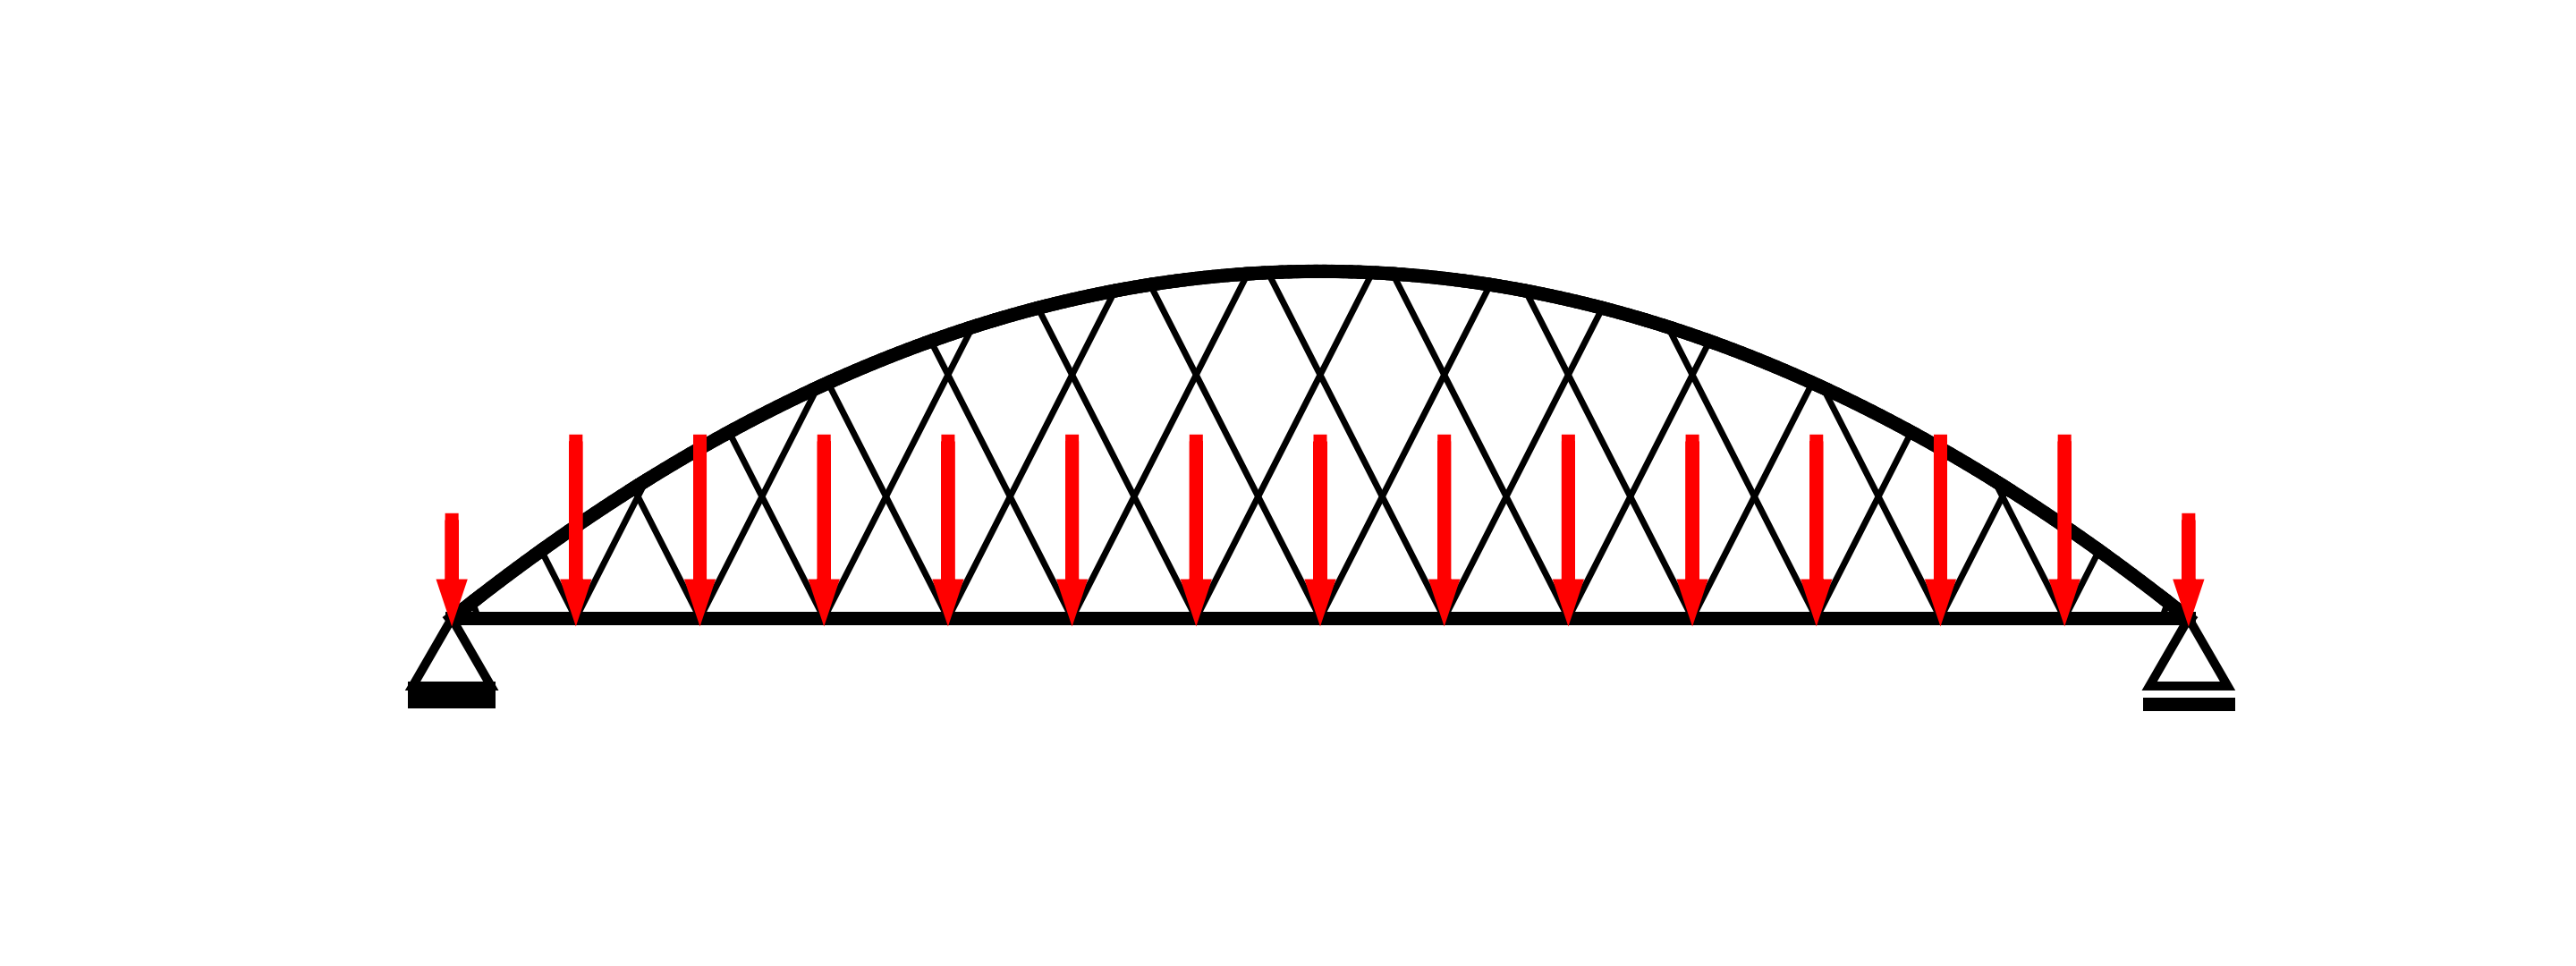
\includegraphics[trim={0 0.8cm 0 0.8cm},clip, width=0.9\textwidth]{illustrations/figures/distributed live loads.png}
    \caption{Distributed live loads}
    \label{fig:Live_load_1}
\end{subfigure}%
\begin{subfigure}{.5\textwidth}
    \centering
    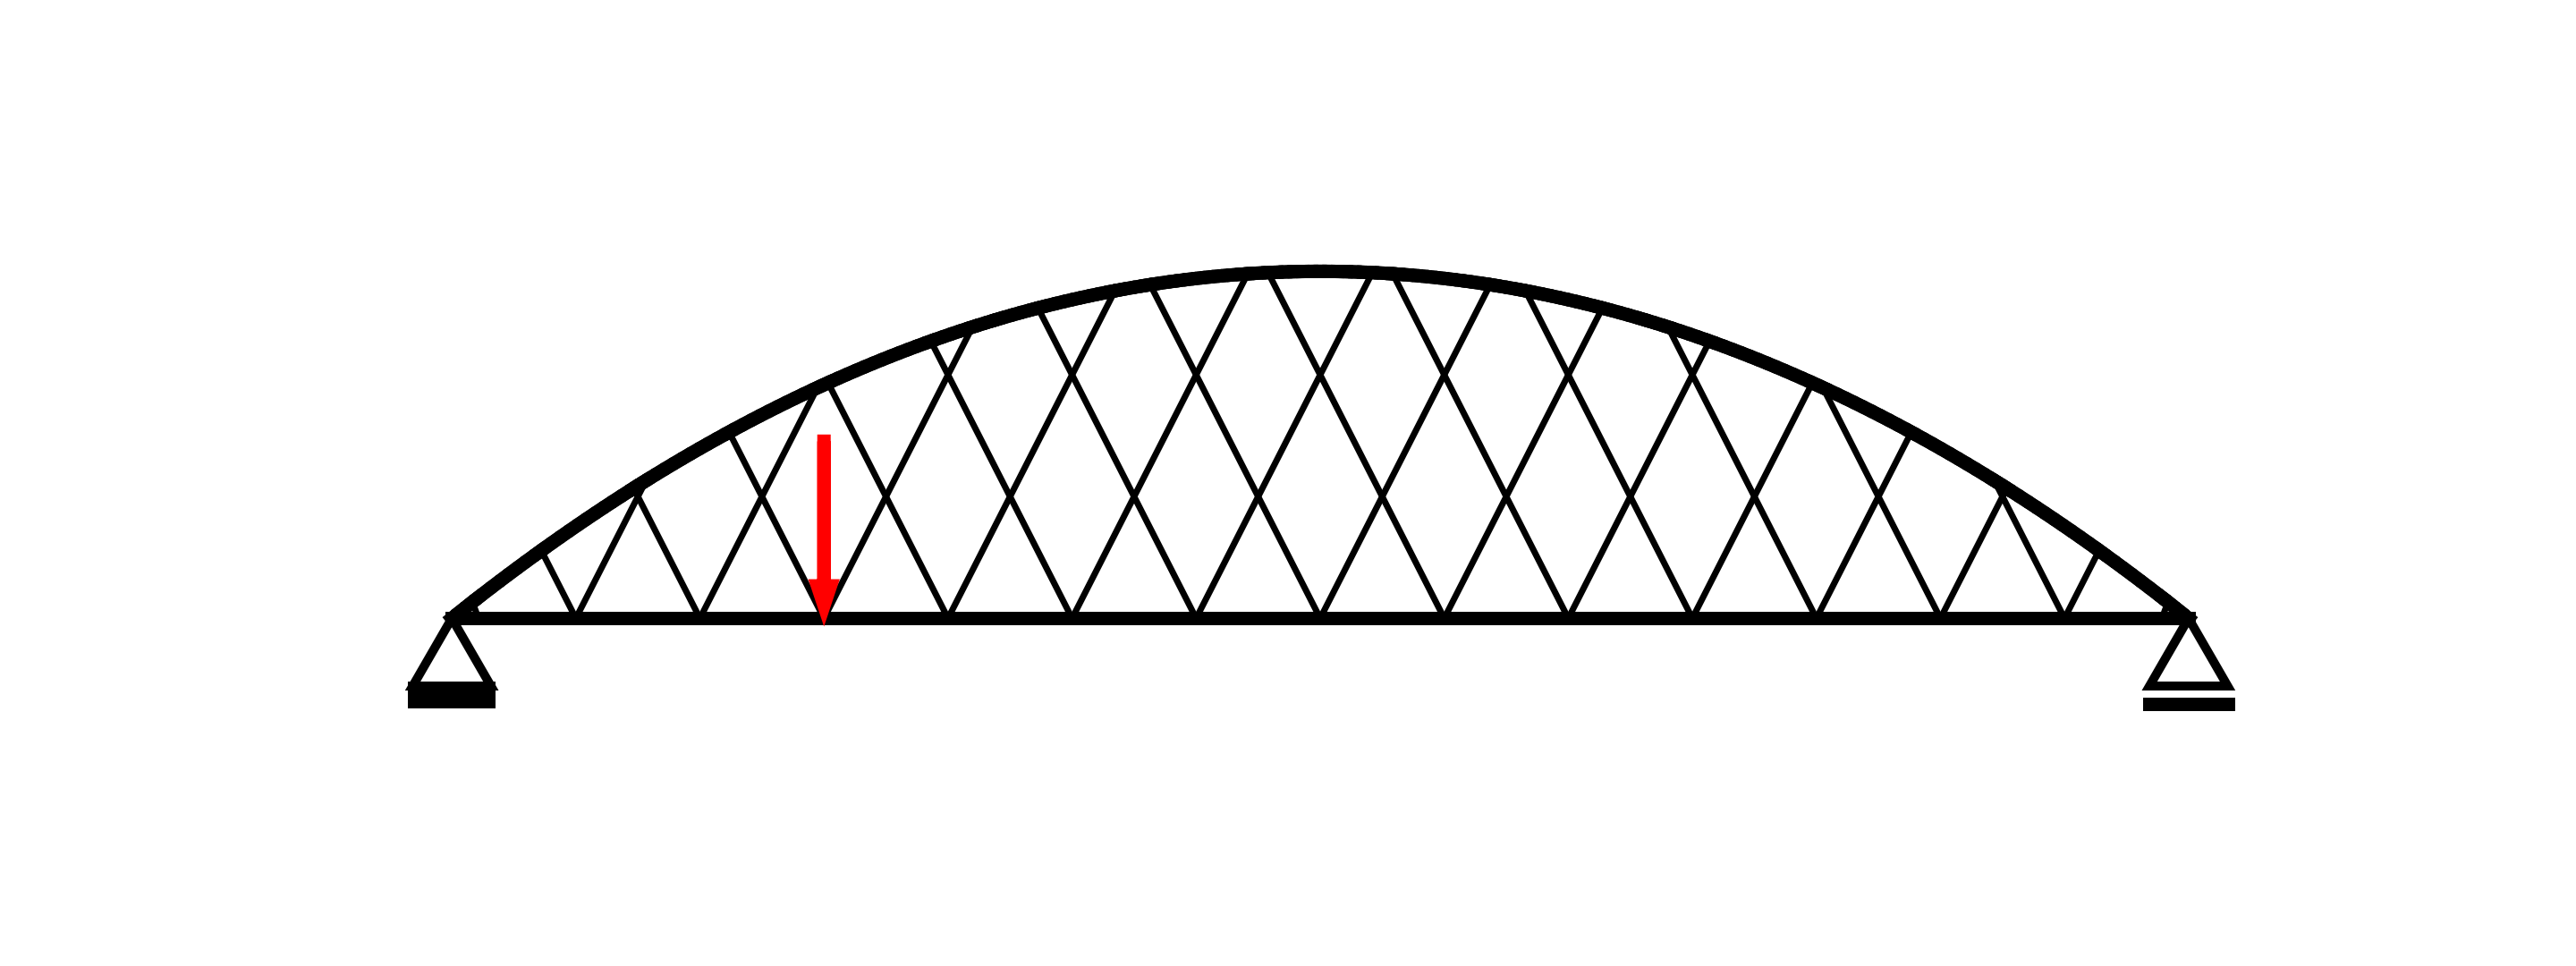
\includegraphics[trim={0 0.8cm 0 0.8cm},clip, width=0.9\textwidth]{illustrations/figures/concentrated live loads.png}
    \caption{Concentrated live loads}
    \label{fig:Live_load_2}
\end{subfigure}
\caption{Live loading in the structural model}
\label{fig:Live_load}
\end{figure}

For the extreme events of cable loss and cable replacement, special circumstances apply to the live loading. For cable loss, it is assumed that only the actually marked lanes are loaded. For cable replacement, one lane is shifted away from the replaced hanger. The determining live load arrangement is also calculated and illustrated in the Appendix \ref{Appendx_A_Live_loading_2}. The resulting loads on the tie are given in Table \ref{tab:live_load_extreme}. For the event of tie fracture, the same live loading as in the ultimate limit states is applied.

\begin{table}[H]
\centering
\caption{Live loads for extreme events}
\label{tab:live_load_extreme}
\begin{tabular}{lcc}
\hline
Extreme event     & Distributed live load & Concentrated live load \\ \hline
Cable loss  & \SI{14.2}{kN/m} & \SI{660}{kN} \\
Cable replacement & \SI{18.8}{kN/m} & \SI{874}{kN} \\ \hline
\end{tabular}
\end{table}


For the fatigue limit state, the loading according to the PTI specifications is used \cite{PTI}. It consists of a single design truck without taking into account the dynamic multiplier. The resulting force, which is derived in the Appendix \ref{Appendx_A_Live_loading_2}, is equal to \SI{296}{kN}.



\subsection{Wind loading}
The load case of wind loading is not calculated in this investigation as the loads are particular to a specific design and require a 3-dimensional model and a very detailed investigation. However, the effects specified on the design drawings, shown in the Appendix \ref{app:design_verifications}, are taken to allow for an integral design verification. The respective characteristic internal force effects under wind loading are shown for each segment in Table \ref{tab:effects_wind_load}.

\begin{table}[H] 
\caption{Effects of wind loading per segment}
\label{tab:effects_wind_load}
\centering
\begin{tabular}{lccc}
\hline
Segment & Normal force & Moment-y & Moment-z \\
 & [MN]   & [MNm] & [MNm] \\ \hline
Arch 1 & -7.8 & -0.67 & 10.7\\
Arch 2 & -4.1 & -0.53 & 2.6\\
Arch 3 & -3.9 & 0.12 & 0.11\\
Tie 1 & 7.0 & -1.1 & 5.9\\
Tie 2 & 6.2 & 0.40 & 0.43\\
Tie 3 & 5.3 & 0.70 & 0.79\\
Hangers & 0.48 & - & - \\ \hline
\end{tabular}
\end{table}


%In [] it is mentioned, that the deciding load case for the design of the Blennerhassett Island Bridge is the accidental tie fracture event. It assumes that one of the flanges or the webs of the tie ruptures, which causes immense stresses and strains on the remaining components and also changes the flow of forces. The investigation of this load case lies outside of the scope of this Thesis. Nevertheless, it is indirectly considered in the objective function, which is introduced in Sec. [].

\newpage
\section{Self-equilibrium stress state} \label{sec:met_seq}
% Permanent state
In a n-times statically indeterminate structure, there are n supernumerary forces or moments. These forces are present in the initial configuration even without any applied loads and form the residual stresses. In the case of a network tied-arch bridge these residual stresses can be controlled during the construction by prestressing the hangers and by applying forces to the arch and the tie when the two are closed and locked. The created self stress state is in equilibrium with itself and will be present under all following load cases. Therefore, it can counteract the effects expected in the strength limit states and simplify the design verifications. This self-equilibrium stress state is described by any set of supernumerary forces. For the investigation in this Thesis, the supernumerary forces presented in Figure \ref{fig:super_forces} are used. Besides the normal forces in the hangers also the moments between the arch and the tie as well as the horizontal force at the right knuckle are part of the supernumerary set.

\begin{figure}[H]
    \centering
    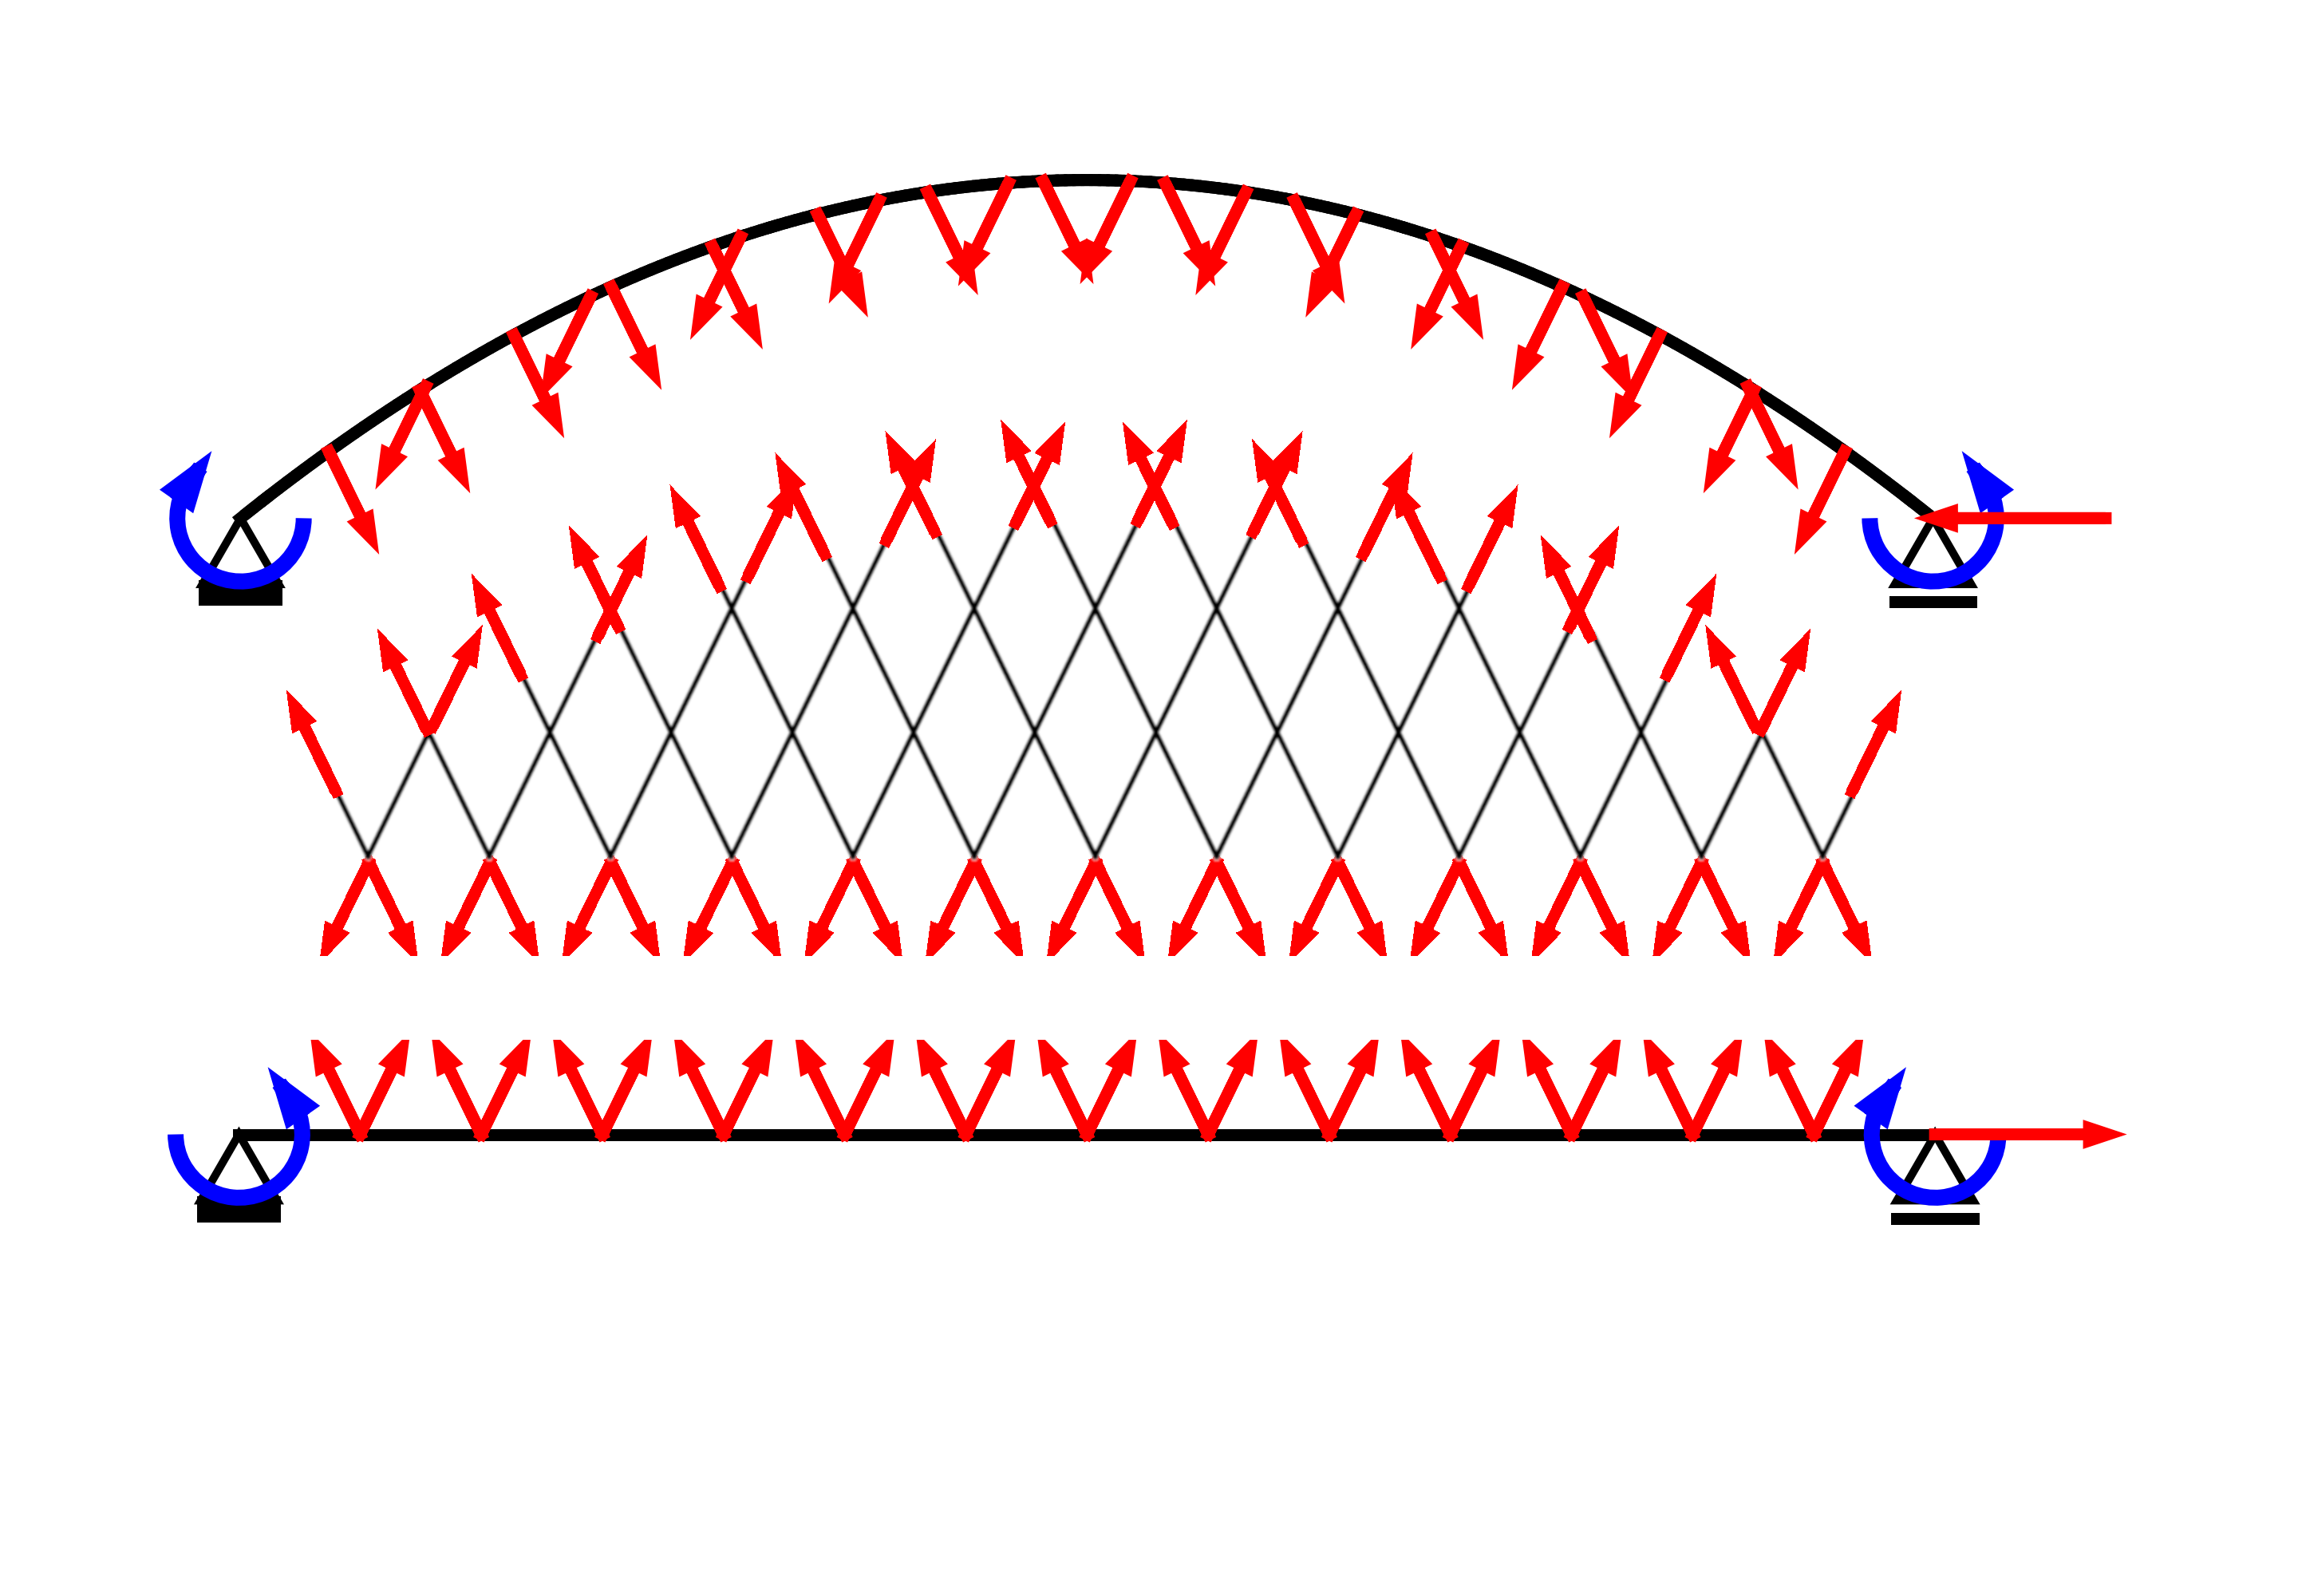
\includegraphics[trim={1cm 16cm 4cm 6.5cm},clip, width=0.65\textwidth]{overleaf/Pictures/Supernumerary forces.png}
    \caption{Set of supernumerary forces in the structural model}
    \label{fig:super_forces}
\end{figure}

For the Blennerhassett Island Bridge, 29 independent self-equilibrium stress states are present, one for each hanger and three for the arch and the tie. Under consideration of symmetry, 15 independent states remain. Instead of the hypothetical residual stress state under no loads, the state under permanent loads is investigated in this Thesis. Thereby, the residual stresses are defined indirectly. 
For the investigation of the stress state under permanent loads, the structural model of the network arch bridge can be split into the tie and the arch. If the forces at the knuckle and in the hangers are consistent, they can ultimately be recombined to form the permanent state of the network arch.
For general circumstances, including unsuitable arch shapes and hanger arrangements, it is a challenging task to find appropriate permanent hanger forces. This task is usually tackled by the engineer through trial and error, as it was the case for the design of the Blennerhassett Island Bridge. The respective result is neither reproducible nor can it claim optimality. In this Section, a few methods with a variety of applications are presented. 


\subsection{Zero-displacement method}
The zero-displacement method gives a first estimation of the hanger forces and is often used for the more popular cable-stayed bridge type. The permanent hanger forces are determined from a structural analysis of the tie girder where at every hanger connection a vertical support is introduced. In this way, the moment distribution in the tie is adequately balanced and creeping effects do not change the moment distribution. For a network tied-arch bridge, additionally to the supports at the connection nodes, a fully fixed support can be introduced at the knuckle. It represents the connection of the tie girder to the arch rib and gives the permanent moment between the two, which has also been considered part of the supernumerary set. The model of the tie resembles a multi span beam, as shown in Figure \ref{fig:zero_disp}. For the case of a network tied-arch bridge, multiple hangers can connect to the tie at a particular node and the vertical forces have to be distributed between the respective hangers. One option is to assign forces of equal magnitude to each of the hangers resulting in the intended vertical force. 

\begin{figure}[H]
    \centering
    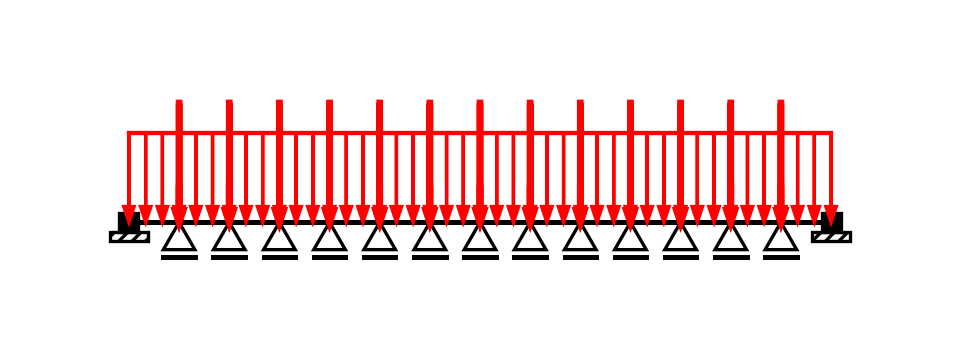
\includegraphics[trim={0 1cm 0 1cm},clip,width=0.6\textwidth]{illustrations/optimisation methods/zero-displacement.png}
    \caption{Zero-displacement method on the tie girder}
    \label{fig:zero_disp}
\end{figure}

In a second step, the hanger forces and the constraint moment at the knuckle are applied to the arch to determine its permanent state. Thereby the arch is affected by a significant moment distribution with the peak at the crown of $M_{p,crown}$. Additionally, the permanent tie tension force, which has a decisive influence on the arch, can be chosen freely at this point as it was neglected in the investigation of the tie girder. As a simplistic approach, the permanent tie tension force $N_{p,Tie}$ can be calculated to cause a disappearing moment at the crown of the arch according to Equation \ref{eq:M_0}. Otherwise, the more elaborate methods in the followings Sections can be used to determine this last supernumerary force.

\begin{equation}
    N_{p,Tie} = \frac{M_{p,crown}}{r}
    \label{eq:M_0}
\end{equation}

This approach is fast and simple to calculate. For a standard hanger arrangement and an adapted arch shape, these simple approaches yield adequate permanent moment distributions. However, for a radial hanger arrangement, in which the hanger connections do not coincide with the floor beams, or for a specific arch shape that does not resemble the respective thrust line, the zero-displacement method does not yield a useful self-equilibrium stress state.

\subsection{Moment minimisation}
It is the goal of an efficient initial configuration to simplify the design verifications by counteracting the effects expected in the various load cases. For the moment minimisation method, this is achieved by minimising the permanent moment distribution in the tie and potentially the arch as well. The permanent moment distribution at m points along the considered component $M \in \mathbb{R}^m$ can be described by Equation \eqref{eq:perm_mom}. 
\begin{equation}
    {\bf M} = {\bf M_0} + \sum_{i=1}^{n} {\bf M_i} \cdot X_i = {\bf M_0} + {\bf M_{sn}} \cdot {\bf X}
    \label{eq:perm_mom}
\end{equation}
where ${\bf M_0} \in \mathbb{R}^m$ is the moment distribution of the permanent loads on the basic system, ${\bf M_i} \in \mathbb{R}^m$ is the moment distribution of the i-th supernumerary unit force, ${X_i} \in \mathbb{R}$ is the i-th supernumerary force. The latter two can be combined into the matrix of supernumerary moment distributions ${\bf M_{sn}} \in  \mathbb{R}^{m\times n}$ and the vector of supernumerary forces or moments ${\bf X} \in \mathbb{R}^n$. An example of a supernumerary hanger force and its moment distribution is shown in Figure \ref{fig:Minimisation}.

\begin{figure}[H]
\centering
\begin{subfigure}{0.5\textwidth}
    \centering
    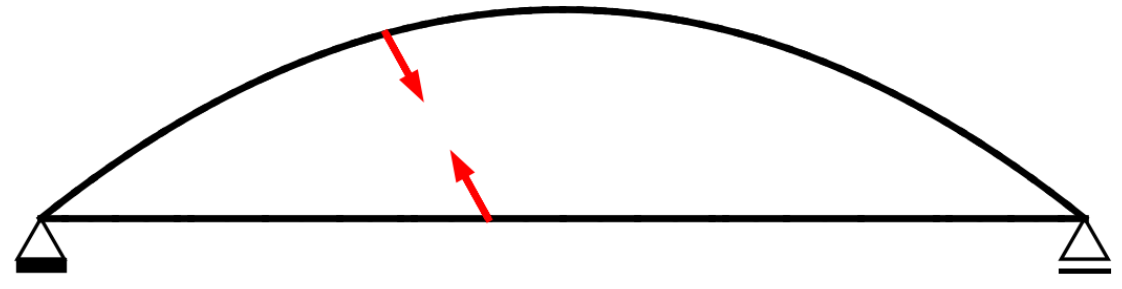
\includegraphics[trim={0 0cm 0 0},clip, width=0.9\textwidth]{overleaf/Appendix/Pictures/min_1.PNG}
    \caption{Basic system and supernumerary force}
    \label{fig:Minimisation_1}
\end{subfigure}%
\begin{subfigure}{.5\textwidth}
    \centering
    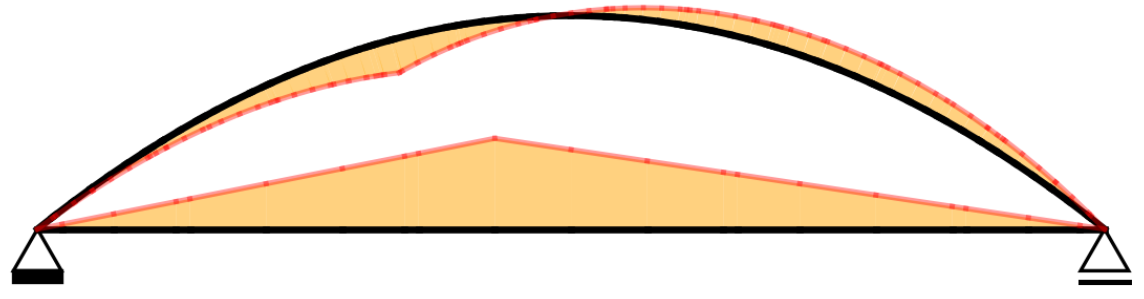
\includegraphics[trim={0 0cm 0 0},clip, width=0.9\textwidth]{overleaf/Appendix/Pictures/min_2.PNG}
    \caption{Moments under supernumerary force}
    \label{fig:Minimisation_2}
\end{subfigure}
\caption{Moment distribution of supernumerary force}
\label{fig:Minimisation}
\end{figure}

\newpage
The problem of minimising the absolute maximum moments can be formulated according to Equation \eqref{eq:minimisation}, where the absolute maximum moment is expressed also as the infinity norm.
\begin{align}
    \underset{{\bf X}}{\text{Minimize}} \quad & f({\bf X}) = \max({\bf M}, -{\bf M}) = \|{\bf M_0} + {\bf M_{sn}} \cdot {\bf X}\|_{\infty} 
    \label{eq:minimisation}
\end{align}
With the helper variable $t$, the previously stated problem can be formulated as a linear programming problem, as shown in Equation \eqref{eq:minimisation_2}.
The variable $t$ describes the moment magnitude which is larger than the all absolute moments in ${\bf M}$ according to the inequality conditions.
\begin{align}
    \underset{t, {\bf X}}{\text{Minimize}} \quad & f(t) = t \label{eq:minimisation_2} \\
    \text{s.t.} \quad & {\bf M_0} + {\bf M_{sn}} \cdot {\bf X} - t {\bf 1} \leq  0 \nonumber \\
    \quad & {-\bf M_0} - {\bf M_{sn}} \cdot {\bf X} - t {\bf 1} \leq 0 \nonumber
\end{align}
Additionally, bounds for the permanent hanger forces can be specified as further inequality conditions. It should be noted that under the consideration of symmetry the amount of variables in the linear problem can be reduced. If only the moment distribution in the tie is optimised, it makes sense to only consider vertical forces at each hanger node to obtain an unambiguous problem. In a second step, the optimised vertical forces are assigned to the two hangers at the node. The obtained problem is efficiently and reliably solvable as it is formulated as a linear programming problem. It can even be solved by Microsoft Excel without the need of additional software.

\subsection{Least squares of moments}
As an alternative approach, the supernumerary forces can be determined using the method of least squares. The objective of this method is to find supernumerary forces which counteract a certain moment distribution, for example the moment distribution on the basic system. Using the variables which were introduced in the previous section, the objective is described by Equation \eqref{eq:lsq_1}.
\begin{equation}
    {\bf M_{sn}} \cdot {\bf X} = -{\bf M_0}
    \label{eq:lsq_1}
\end{equation}
As this yields an overdetermined system, the equations cannot be solved simultaneously. Using the method of least squares, the sum of the squared deviations can be minimised by solving the determined system in Equation \eqref{eq:lsq_2}.
\begin{equation}
    ({\bf M_{sn}}^T\,{\bf M_{sn}}) \cdot {\bf X} = -{\bf M_{sn}}^T\,{\bf M_0}
    \label{eq:lsq_2}
\end{equation}
The drawback of this method is that no bounds for the hanger forces can be specified. However, this method is particularly useful, if the hanger forces have been optimised by minimising the moments on the tie girder. At this point, the permanent tension force in the tie girder is still undefined, as it does not affect the moment distribution. It can then be calculated by considering the moment distribution in the arch rib, minimising the squares of its moment distribution. In this case, the approach is fast and can even be solved without using linear algebra as there is only one variable.


\newpage
\section{Arch shape} \label{sec:met_arch}
The optimisation methods which were introduced in the previous chapter allow finding an efficient self-equilibrium stress state for a given arch shape. This corresponds to finding hanger forces with a resulting thrust line close to the predefined arch shape. However, a more elegant solution would be an adaptation of the arch shape to the thrust line under permanent loads. There are two thrust line derivations relevant for this Thesis. In Section \ref{app:continuous}, the thrust line is derived for the hypothetical case of an infinitely dense hanger arrangement. For a discrete hanger arrangement the thrust line can be derived according to the method described in Section \ref{app:discrete}. Both methods take the weight of the arch into account.

\subsection{Thrust line of continuous hanger arrangement}\label{app:continuous}
In a first step, the hanger force densities of each hanger set are determined without the consideration of the arch. There are multiple possibilities to do so. For example, they could be calculated to be in equilibrium with the permanent vertical force $q$, depending on their angles of inclination $\alpha$ and $\beta$. However, horizontal equilibrium is an unnecessary condition, as the tie is affected by significant tension forces anyway. Therefore, it is proposed to assign force densities of identical magnitude to hangers on each infinitesimal element, as illustrated in Fig. \ref{fig:continuous_1}. Also the resultant forces $F_L$ and $F_R$ are shown.
\begin{figure}[H]
    \centering
    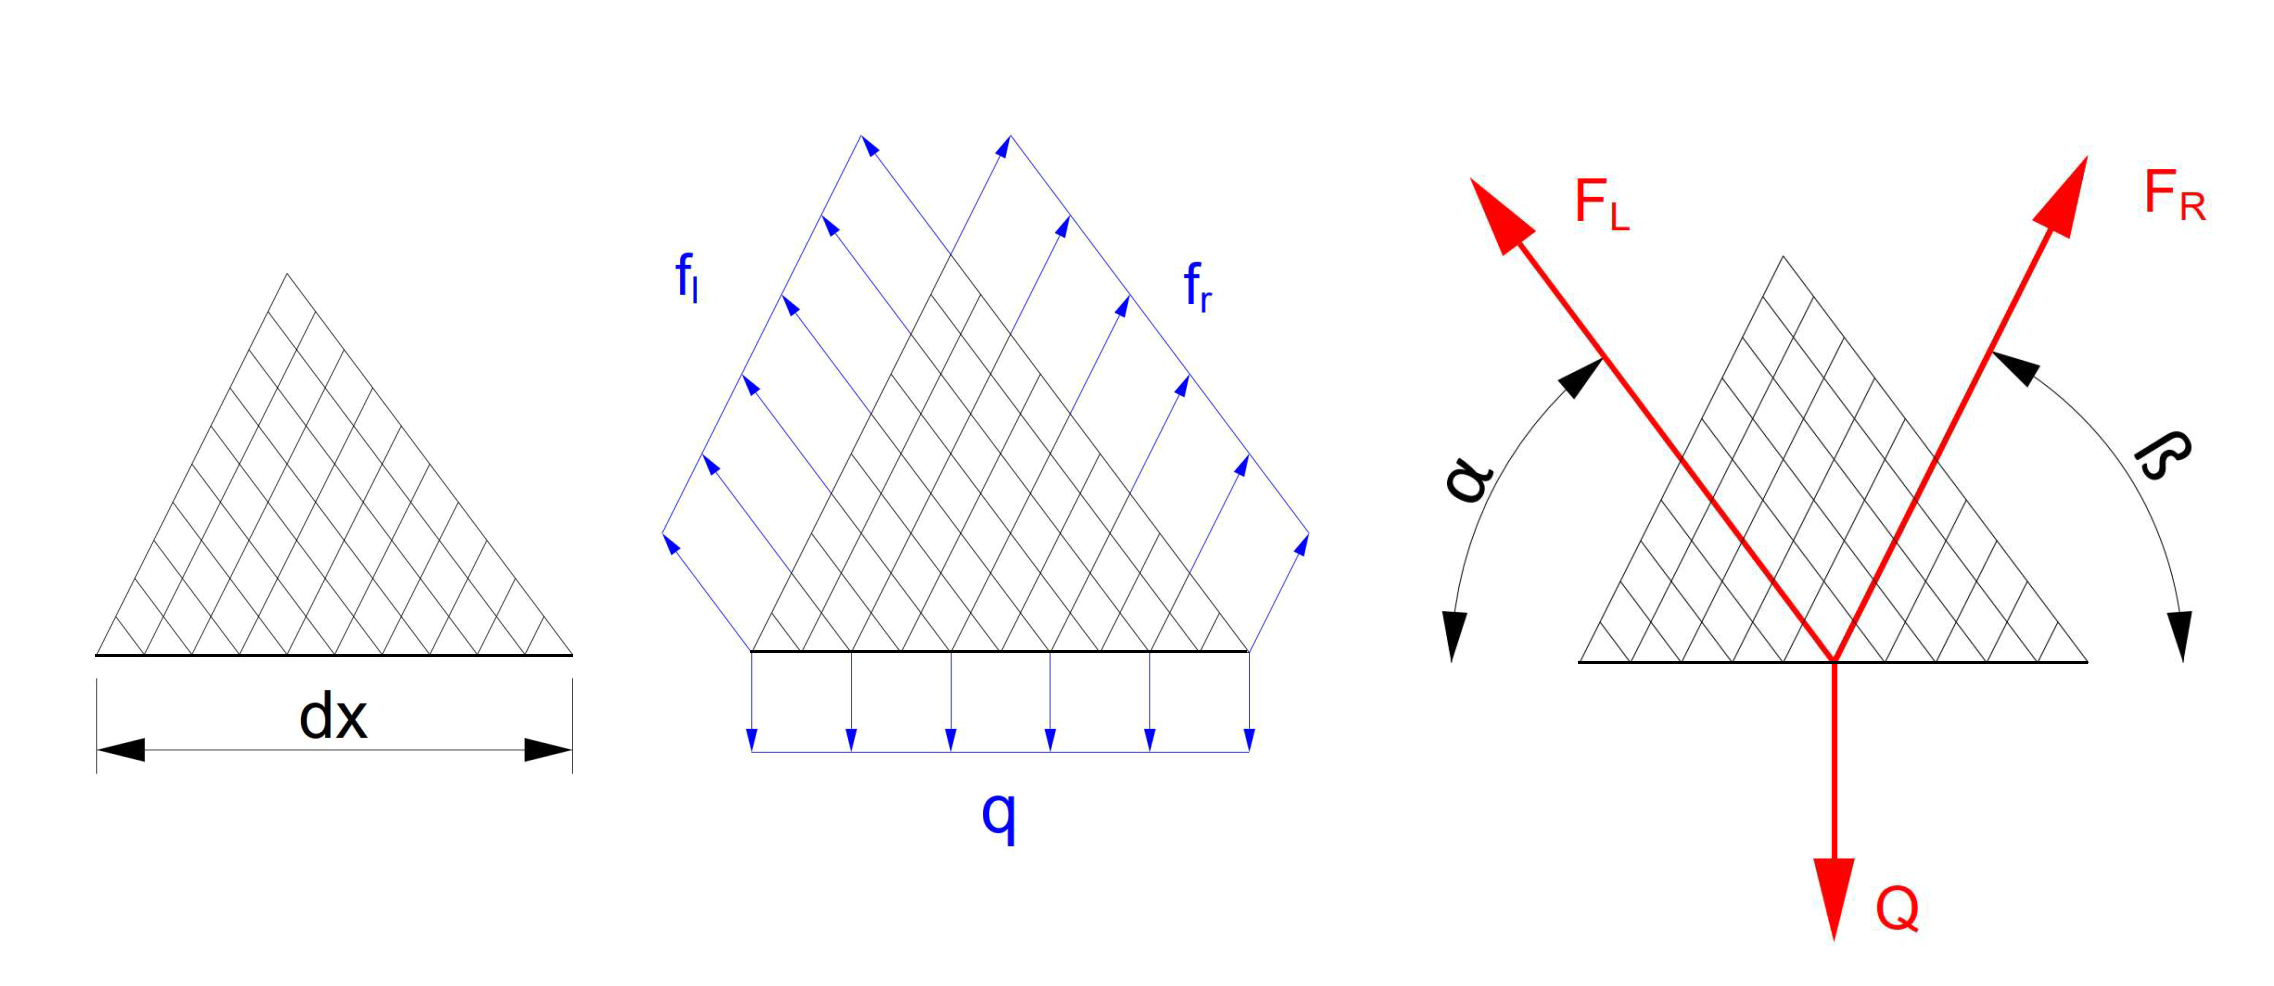
\includegraphics[width=0.8\textwidth]{overleaf/Appendix/Pictures/continuous_thrust_line_1.PNG}
    \caption{Hanger force densities on an infinitesimal element}
    \label{fig:continuous_1}
\end{figure}

The corresponding hanger force densities $f_l$ and $f_r$ can be calculated according to Eq. \eqref{eq:continuous_1}.
\begin{equation}
    f_l=f_r=\frac{q}{\sin{\alpha}+ \sin{\beta}}
    \label{eq:continuous_1}
\end{equation}

While the thrust line can be described analytically by a differential equation, it is impossible to get an analytical solution for general hanger arrangement patterns. Therefore, the thrust line of the infinitesimal hanger arrangement is calculated in fixed horizontal steps of $dx$ starting from the crown, where a normal force $N_{crown}$ is assumed. If the step $dx$ is small, it can be assumed, that the inclination of the thrust line undergoes small changes in every step. At the beginning of each step the normal force $N_1$ is known, which also corresponds to the inclination of the thrust line. In each step, the change of height of the thrust line $dy$ is determined iteratively. It underlies the condition that the new inclination coincides with the inclination of the new normal force, which can be described by Eq. \ref{eq:continuous_2}.
\begin{equation}
    dy = \frac{dx}{2} \cdot \left(\frac{N_{1,y}}{N_{1,x}} + \frac{N_{2,y}}{N_{2,x}} \right)
    \label{eq:continuous_2}
\end{equation}

The new normal force $N_2$ is determined from force equilibrium considering the hanger forces and the self weight, both of which depend on $dy$. The self weight is determined from the length of the segment multiplied by the weight per meter. For the hanger forces, the lengths of the two hanger sets on the tie $dl_1$ and $dl_2$ affecting the considered arch segment are determined over geometrical considerations. Using the previously determined hanger force densities the resulting hanger force is determined. The calculation of a single step is illustrated in Fig. \ref{fig:continuous_2}.
\begin{figure}[H]
    \centering
    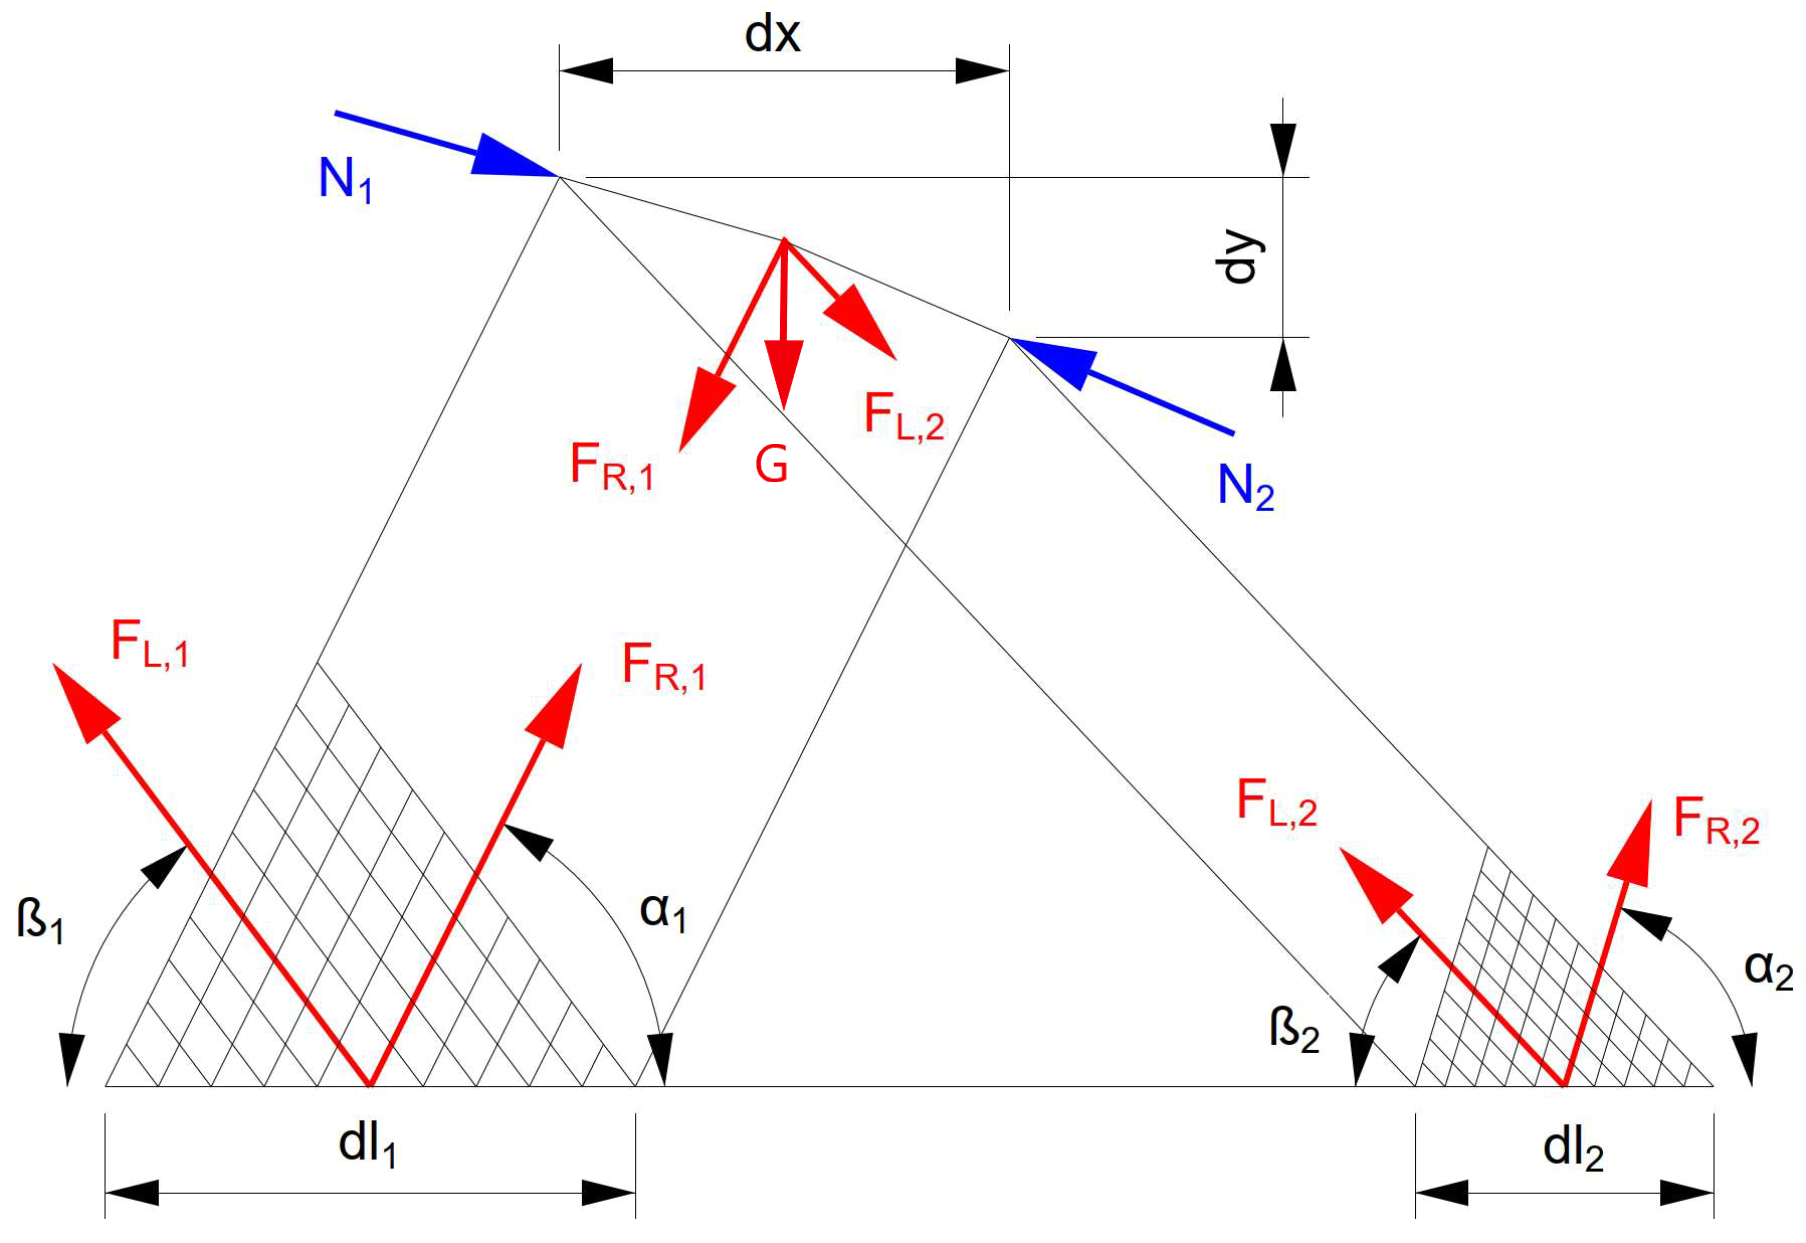
\includegraphics[width=0.6\textwidth]{overleaf/Appendix/Pictures/continuous_thrust_line.PNG}
    \caption{Derivation of the arch thrust line for a continuous hanger arrangement}
    \label{fig:continuous_2}
\end{figure}

Ultimately, the normal force in the crown $N_{crown}$ is determined iteratively for the thrust line to intersect the knuckle point. However, this normal force in the crown could also be determined from static considerations involving global longitudinal moment and the hanger force densities without the need of an iteration.


\subsection{Thrust line of discrete hanger arrangement}\label{app:discrete}

Calculating the thrust line of a discrete hanger arrangement is a particular challenge as it is not known in which order the hangers intersect the thrust line beforehand. Therefore it is also calculated in steps. Similar to the continuous calculation, it is started from the crown with an estimated normal force $N_{crown}$ and the inclination at the beginning of every step corresponds to the ratio of the normal force components. Further, the arch's weight per horizontal meter is estimated from Eq. \ref{eq:g_arch}.

\begin{equation}
    g_{arch,x} = g_{arch} \cdot \sqrt{1+y'^2} = g_{arch} \cdot \sqrt{1+\left( \frac{N_{y}}{N_{x}} \right)^2}
    \label{eq:g_arch}
\end{equation}

Using this weight per horizontal meter, the parabolic thrust line can be estimated according to Eq. \ref{eq:discrete}. The height at the beginning of the current step is given by $y_1$ The second term gives the inclination of the normal force, which would continue the thrust line under no additional loading. The weight of the arch causes a slight curvature according to the third quadratic term.

\begin{equation}
    y(x) = y_1 - \frac{N_y}{N_x} \cdot x - \frac{g_{arch,x}}{2\cdot N_x}\cdot x^2
    \label{eq:discrete}
\end{equation}

Unless a hanger intersects the thrust line within the current step, the thrust line is continued by the step length $dx$. An illustration is given in Fig. \ref{fig:discrete_1}.

\begin{figure}[H]
    \centering
    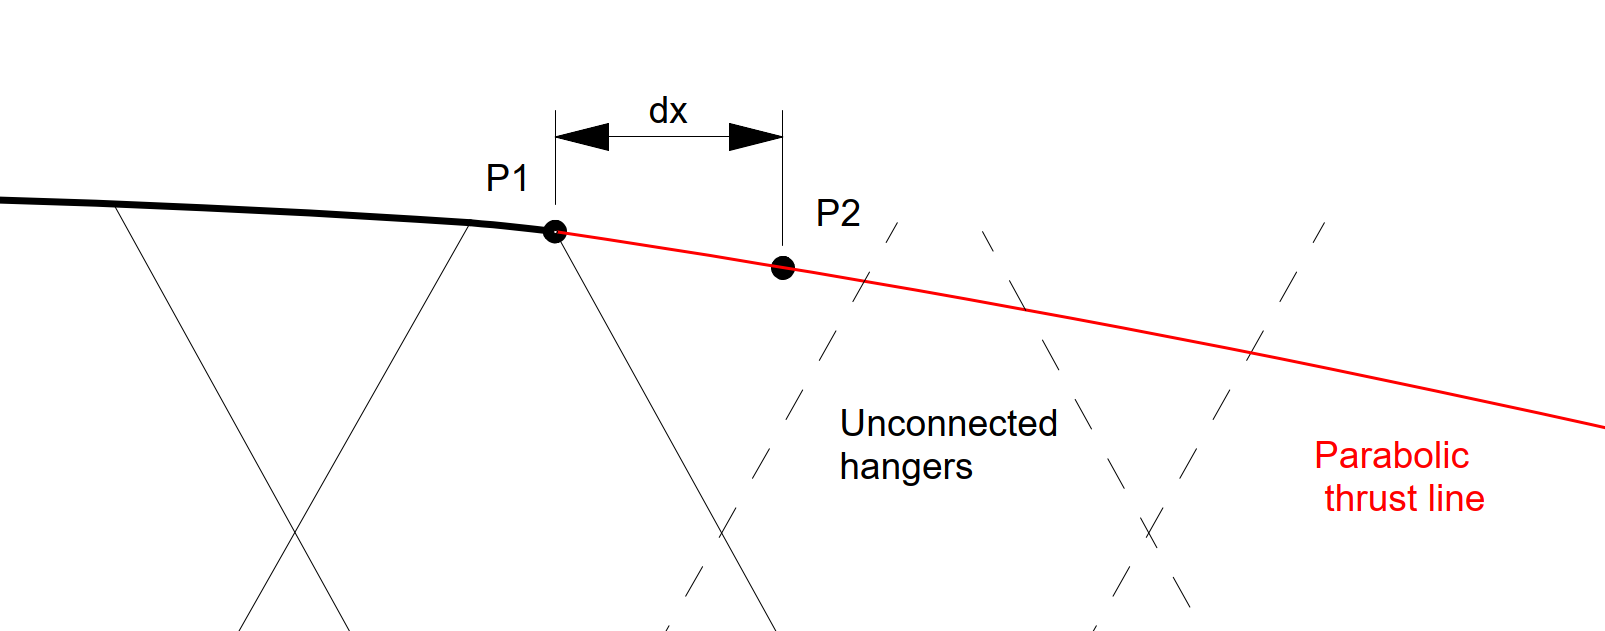
\includegraphics[width=0.7\textwidth]{overleaf/Appendix/Pictures/discrete_thrust_line_1.PNG}
    \caption{Thrust line derivation step without intersecting hangers}
    \label{fig:discrete_1}
\end{figure}

However, if a hanger intersects the thrust line within the current step, this intersection point is added to the thrust line and used as a starting point for the next step. This step is illustrated in Fig. \ref{fig:discrete_2}.

\begin{figure}[H]
    \centering
    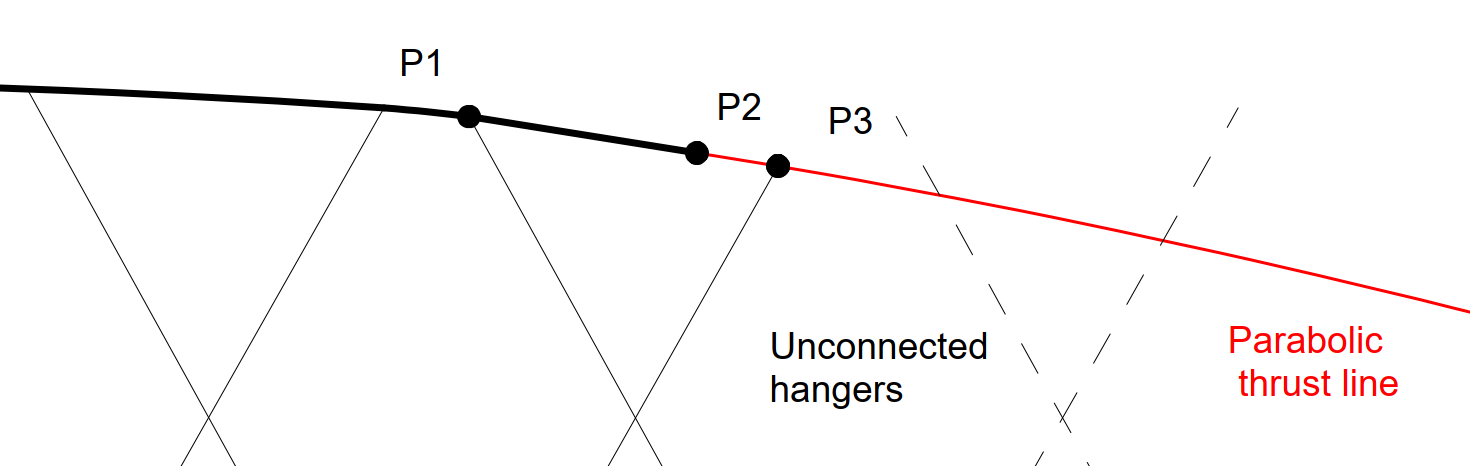
\includegraphics[width=0.7\textwidth]{overleaf/Appendix/Pictures/discrete_thrust_line_2.PNG}
    \caption{Thrust line derivation step connecting to the next hanger}
    \label{fig:discrete_2}
\end{figure}

Again, the normal force in the crown $N_{crown}$ is determined iteratively for the thrust line to intersect the knuckle point. Numerically, it would be much easier to calculate it from static considerations.

\subsection{Polynomial approximation}

\newpage
\section{Design verifications} \label{sec:met_ver}
To ensure a safe and reliable structure, the limit states for strength, extreme events and fatigue are considered \cite{AASHTO}.  The resulting demand over capacity ratios (D/C) will also be used in Section \ref{sec:met_cost} for an estimation of the cost function.

\subsection{Strength limit states}
The strength limit states are considered to ensure that the design of the structure guarantees enough strength and stability for the highest expected loads in its life cycle. The load combinations considered in this investigation are related to the main actions of vehicular use (Strength-I), wind exposure (Strength-III) and a load combination for heavy bridges (Strength-IV). The load factors used for each strength limit state are presented in Table \ref{tab:uls_combination}. For the permanent loads DC and DW, two factors are given out of which the one impeding to the verification is taken. For the locked-in erection stresses no variability is taken into account.

\begin{table}[H]
\caption{Load combinations for the ultimate limit state}
\centering
\begin{tabular}{lccccc}
\hline
Load         & EL  & DC         & DW         & LL   & WS  \\ \hline
Strength-I   & 1.0 & 0.9 / 1.25 & 0.65 / 1.5 & 1.75 & -   \\
Strength-III & 1.0 & 0.9 / 1.25 & 0.65 / 1.5 & -    & 1.4 \\ 
Strength-IV  & 1.0 & 0.65 / 1.5 & 0.65 / 1.5 & -    & - \\ \hline
\end{tabular}
\end{table}

The arch and the tie are verified according to Equation \eqref{eq:design_verification}, neglecting the secondary force effects. For the hangers, enough resistance is proved if the highest stresses are below 65\% of the nominal capacity. 

\begin{equation}
    \frac{N_{Ed}}{N_{Rd}} + \frac{8.0}{9.0}\, \left(\frac{M_{y,Ed}}{M_{y,Rd}}+\frac{M_{z,Ed}}{M_{z,Rd}} \right) \leq 1.0
    \label{eq:design_verification}
\end{equation}

For simplicity, the value given by the left side of this condition is also referred to as the demand over capacity ratio for the arch and the tie.
%For the Blennerhassett Island Bridge, the DOC is evaluated according to this simplified verification. The obtained values are presented in Table [], along with the ratios taken from the design drawings in parenthesis. 

\subsection{Extreme event limit states}
Extreme events are unique circumstances whose return periods can be significantly greater than the life expectancy of the structure. In these events, the requirement for the bridge is its structural survival. In this investigation the extreme events of cable loss, cable replacement and tie fracture are examined. The load factors for each event is taken from the design drawings and presented in Table \ref{tab:extreme_combination}. For the events of cable loss and cable replacement, specific live loading arrangements (LL*) apply.

\begin{table}[H]
\caption{Load combinations for the extreme event limit states}
\label{tab:extreme_combination}
\centering
\begin{tabular}{lccccc}
\hline
Event         & EL  & DC         & DW         & LL*   & DAF  \\ \hline
Cable loss   & 1.0 & 1.2 & 1.4 & 0.75 & 1.75   \\
Cable replacement & 1.0 & 1.2 & 1.4 & 1.5 & 1.0 \\ 
Tie fracture  & 1.0 & 1.25 & 1.5 & 1.3 & - \\ \hline
\end{tabular}
\end{table}

For both hanger-related extreme events, each hanger is investigated individually according to the PTI (static) approach [cite PTI]. In a first step, the longitudinal live load arrangement, which maximises the respective hanger force, is determined. Therefor, The concentrated live load is always applied at the cross-girder closest to the considered hanger. The forces from the distributed live load are also arranged on a certain amount of neighbouring cross-girders, as illustrated in Figure \ref{fig:Cable_Loss_1}. The assumed hanger force before its replacement or loss is thereby determined. In a second step, the structural system is modified by removing the considered hanger. The hanger force is applied in opposite direction on the modified system, as shown in Figure \ref{fig:Cable_Loss_2}. The resulting effects are multiplied by a dynamic amplification factor (DAF) and superimposed on the effects from the state of maximised hanger force. The DAF for the event of cable loss is assumed to be 1.75.

\begin{figure}[H]
\centering
\begin{subfigure}{0.5\textwidth}
    \centering
    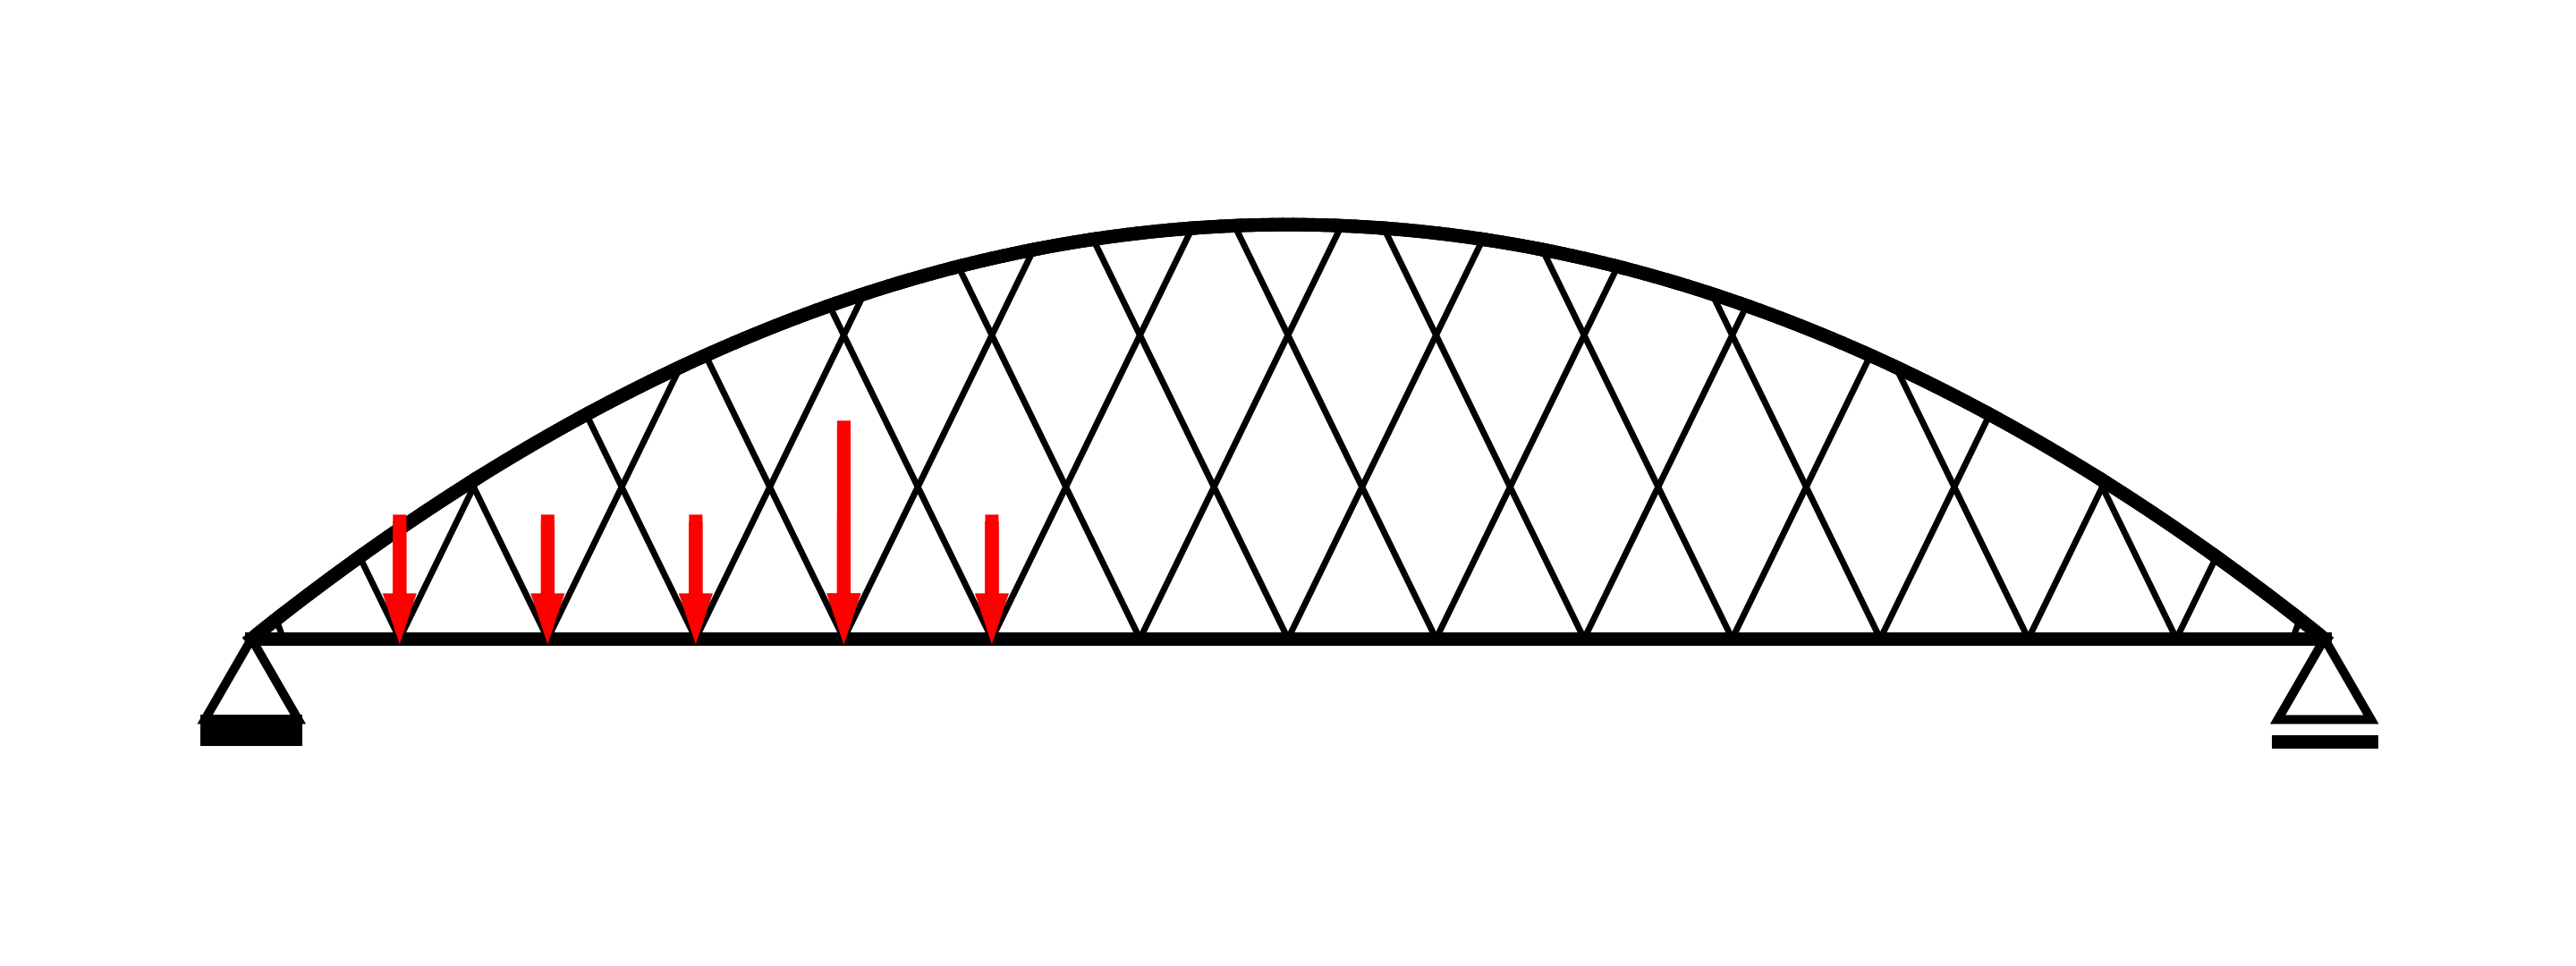
\includegraphics[trim={0 0.8cm 0 0.8cm},clip, width=0.9\textwidth]{illustrations/figures/cable loss - load arrangement.png}
    \caption{Live load arrangement to maximise hanger force}
    \label{fig:Cable_Loss_1}
\end{subfigure}%
\begin{subfigure}{.5\textwidth}
    \centering
    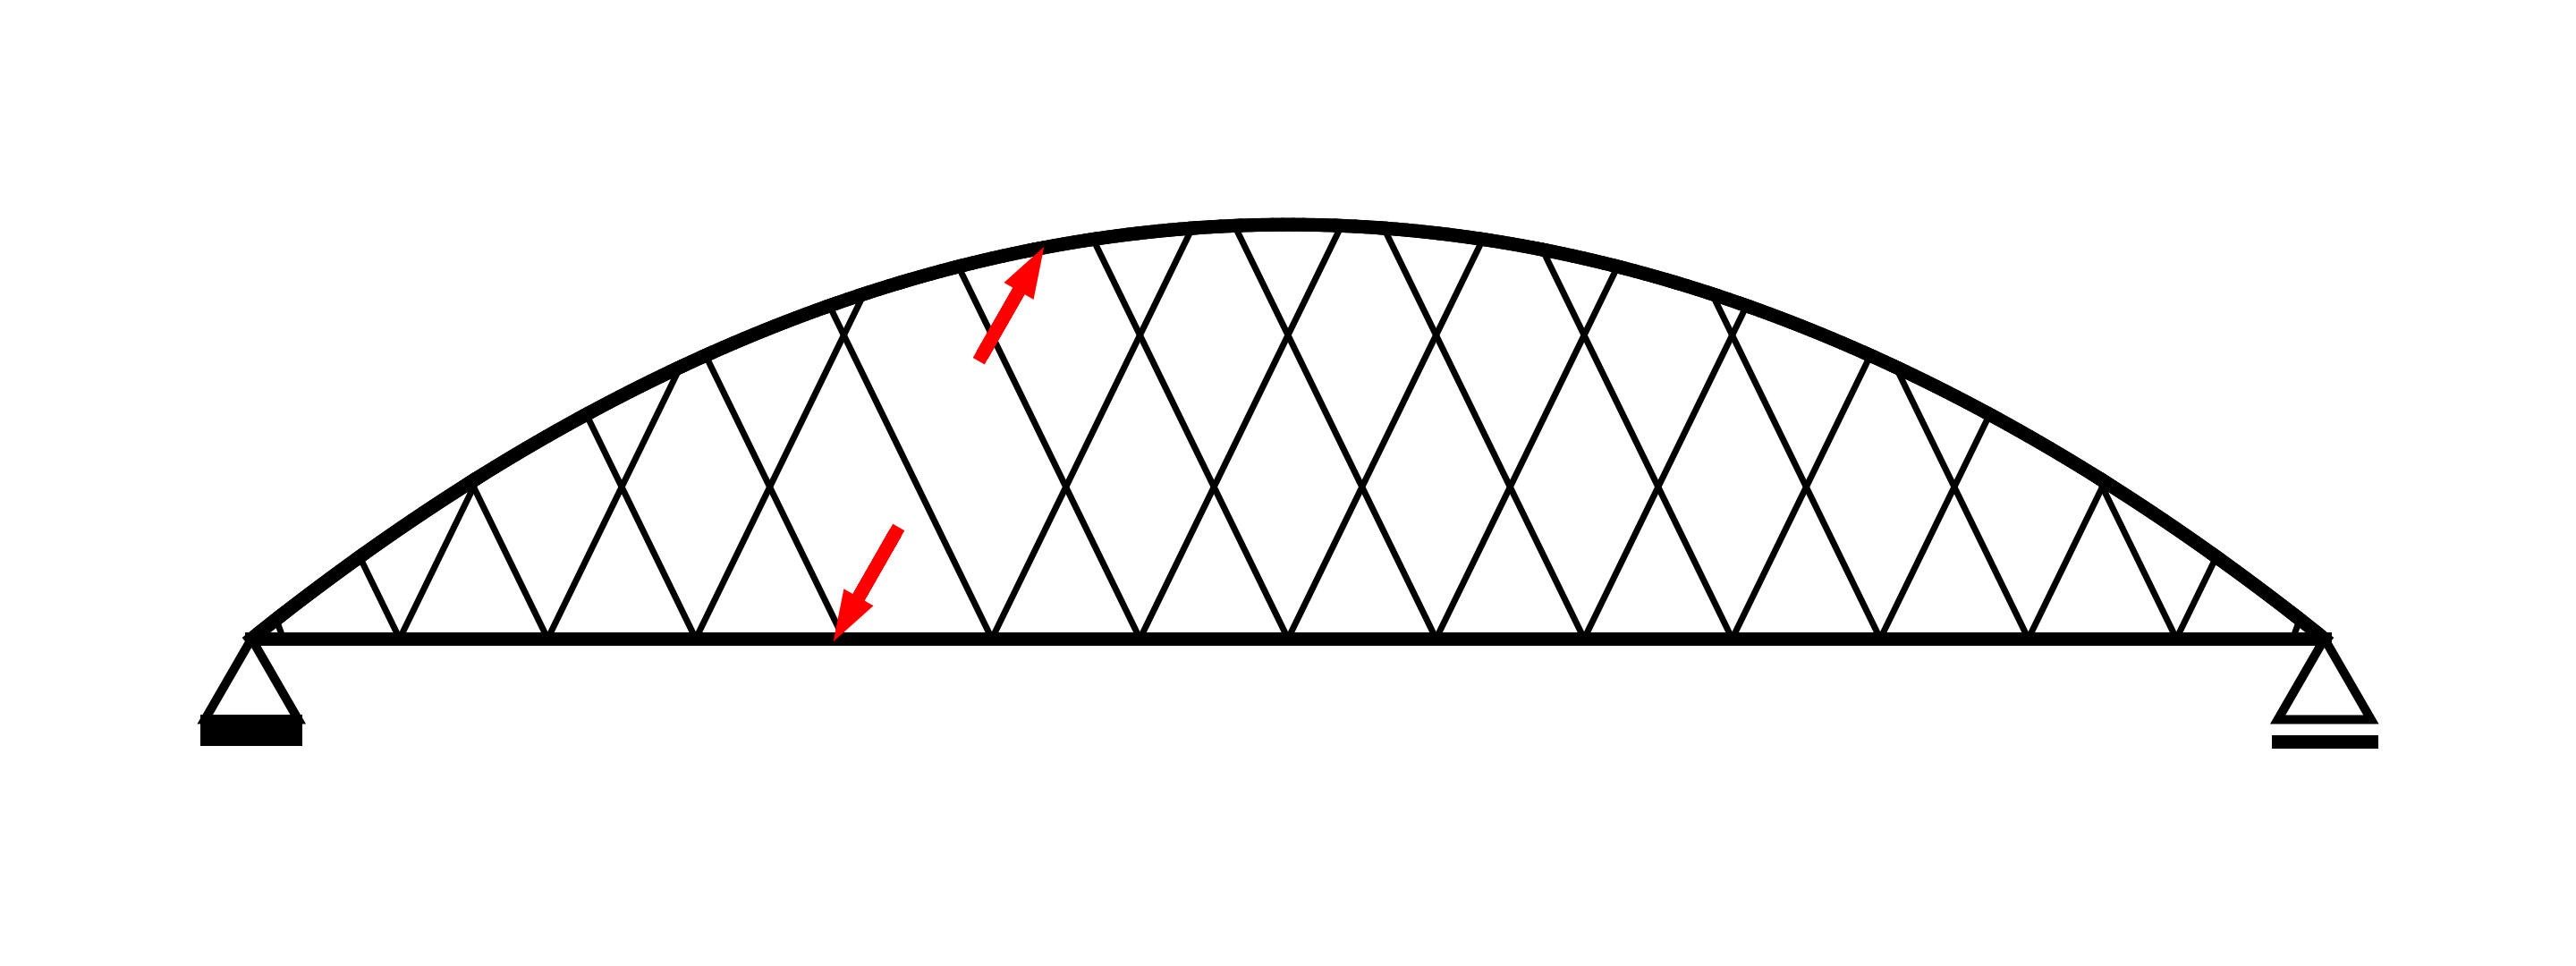
\includegraphics[trim={0 0.8cm 0 0.8cm},clip, width=0.9\textwidth]{illustrations/figures/cable loss.png}
    \caption{Structural model with opposite force}
    \label{fig:Cable_Loss_2}
\end{subfigure}
\caption{Calculation steps for loss of the fourth hanger}
\label{fig:Cable_Loss}
\end{figure}

[Tie fracture]

\subsection{Fatigue limit state}

\begin{table}[H] 
\caption{Cross-sectional resistances}
\centering
\begin{tabular}{lccc}
\hline
Segment & Normal force & Moment-y & Moment-z \\
 & [MN]   & [MNm] & [MNm] \\ \hline
Arch 1 & \SI{130.0}{} & \SI{78.7}{} & \SI{79.1}{}\\
Arch 2 & \SI{108.8}{} & \SI{71.5}{} & \SI{63.4}{}\\
Arch 3-4 & \SI{82.3}{} & \SI{50.0}{} & \SI{42.7}{}\\
Tie 1 & \SI{153.2}{} & \SI{100.8}{} & \SI{76.2}{}\\
Tie 2 & \SI{117.1}{} & \SI{82.8}{} & \SI{56.6}{}\\
Tie 3-4 & \SI{100.6}{} & \SI{76.2}{} & \SI{45.8}{}\\
Hangers & 4.19 & - & - \\\hline
\end{tabular}
\end{table}

\section{Estimation of cost function} \label{sec:met_cost}
